% !TeX root = ../libro.tex
% !TeX encoding = utf8


\chapter{Análisis de Redes Convolucionales}\label{ch:analisis}

\section{Introducción}


\noindent En el contexto del procesamiento de imágenes, se define el término \textbf{invarianza} como la capacidad de reconocer un objeto en la imagen incluso si su apariencia ha variado en algún sentido (rotando, deformando ligeramente o trasladando el objeto por ejemplo). Esto es algo muy importante y positivo, pues esto indica que se preserva la identidad del objeto incluso a pesar de haberse sometido a ciertos cambios.

\medskip

\noindent Las simetrías e invarianzas, aunque juegan un papel más importante en el campo de la Física, van abriéndose paso en el procesamiento de información de señales. La información contenida en las señales referente a imágenes o sonidos no suele verse afectada bajo la acción de grupos finitos como las traslaciones o las rotaciones, y es estable a la acción de pequeños difeomorfismos que deforman las señales. Esto motiva el estudio de las representaciones de traslaciones e invarianzas de las funciones de $L^2(\mathbb{R}^d)$, que son Lipschitz-continuas por la acción de difeomorfismos y que mantienen información de alta frecuencia para diferenciar entre distintos tipos de señales. 

\medskip

\noindent En primer lugar nos centraremos en la invarianza por traslaciones, entendida en el contexto de las imágenes como trasladar cada pixel de la imagen en una misma dirección la misma distancia. En este sentido: 
\begin{definicion}
$L_cf(x)=f(x-c)$ es la traslación de $f \in L^2(\mathbb{R}^d)$ por $c \in \mathbb{R}^d$ .
\end{definicion}

\noindent Así, decimos que un operador $\Phi$ de  $L^2(\mathbb{R}^d)$ en un espacio de Hilbert $\mathcal{H}$ es invariante por traslaciones si $\Phi(L_cf(x))=\Phi(f)$ para todo $f \in L^2(\mathbb{R}^d)$ y para todo $c \in \mathbb{R}^d$. El módulo de la transformada de Fourier de $f$ es un ejemplo de un operador invariante por traslaciones no canónico que estudiaremos en la sección siguiente. 

\medskip

\noindent Sin embargo, estos operadores invariantes a traslaciones no son Lipshcitz-continuos por la acción de difeomorfismos. Es conocido el hecho de que aparecen inestabilidades frente a deformaciones en las altas frecuencias, y el mayor reto es preservar la Lipschitz-continuidad en esta situación.

\medskip

\noindent Para preservar la estabilidad en $L^2(\mathbb{R}^d)$ queremos que $\Phi$ sea no-expansiva. 

\begin{definicion}
Decimos que $\Phi$ es no-expansiva si: 
$$\forall (f,h) \in L^2(\mathbb{R}^d)^2 \; || \Phi(f)-\Phi(h)||_\mathcal{H} \leq ||f-h||$$
\end{definicion}

\noindent Es entonces suficiente verificar su Lipschitz-continuidad relativa a la acción de pequeños difeomorfismos cercanos a las traslaciones. Dichos difeomorfismos transforman $x \in \mathbb{R}^d$ en $x-\tau (x)$ dónde $\tau$ es el campo de desplazamiento. 

\begin{definicion}
Denotemos $L_{\tau} f(x)=f(x-\tau(x))$ como la acción del difeomorfismo $\mathbb{1}-\tau$ en $f$.
\end{definicion} 

\medskip

\noindent La condición de Lipschitz nos dice que $||\Phi(f)-\Phi(L_\tau f)||$ está acotada por el "tamaño" del difeomorfismo, y por tanto por la distancia entre $\mathbb{1}-\tau$ y $\mathbb{1}$, hasta $||f||$ por una constante multiplicativa. 

\medskip

\noindent Sea $|\tau (x)|$ la norma euclídea en $\mathbb{R}^d$, $\nabla |\tau (x)|$ la norma del supremo de la matriz $\nabla \tau (x)$, y $|H \tau (x)|$ la norma del supremo del tensor Hessiano.  

La topología débil (recordemos que es la topología menos fina de un espacio normado que hace continuas todas las aplicaciones de su dual) en los difeomorfismos $C^2$  permite definir la siguiente aplicación: 
\begin{definicion}
Así, se define una distancia entre $\mathbb{1}-\tau$ y $\mathbb{1}$ en cualquier subconjunto compacto $\Omega$ de $\mathbb{R}^d$ como 

$$(1.1) \; \; d_\Omega(\mathbb{1},\mathbb{1}-\tau) = \sup_{x \in \Omega} |\tau (x)| + \sup_{x \in \Omega} |\nabla \tau (x)| + \sup_{x \in \Omega}|H \tau (x)|  $$
\end{definicion}
\medskip

\begin{definicion}
\noindent Un operador invariante por traslaciones $\Phi$ se dice \entrecomillado{Lipchitz-continuo} por la acción de los difeomorfismos $C^2$  si para cualquier compacto $\Omega \subset \mathbb{R}^d$ existe una constante $C$ tal que para todo $f \in L^2(\mathbb{R}^d)$ con Soporte en $\Omega$ y para todo $\tau \in C^2(\mathbb{R}^d)$ se cumple:

$$(1.2)  \; \; || \Phi(f)-\Phi(L_{\tau}f)||_\mathcal{H} \leq C||f||(\sup_{x \in \mathbb{R}^d} |\nabla \tau (x)| + \sup_{x \in \mathbb{R}^d}|H \tau (x)|)$$

\end{definicion}

\medskip

\noindent Debido a que $\Phi$ es invariante a traslaciones, la cota superior de Lipschitz no depende de la amplitud máxima de traslación $\sup_x|\tau (x)|$ de la métrica del difeomorfismo (1.1). Por otro lado la continuidad Lipschitz de (1.2) implica que $\Phi$ es invariante por traslaciones globales, pero es mucho más fuerte. $\Phi$ se ve poco afectada por los términos de primer y segundo grado de difeomorfismos que son traslaciones locales.

\medskip

\noindent Las inestabilidades por altas frecuencias de las deformaciones se pueden evitar agrupando las frecuencias en paquetes diádicos en $\mathbb{R}^d$ con transformadas de ondeletas. Sin embargo, una transformada de ondeletas no es invariante por traslaciones. Es posible construir un operador invariante por traslaciones mediante un procedimiento de dispersión a lo largo de múltiples caminos, que preservan la condición de lipschitz de las ondeletas por la acción de difeomorfismos. Un propagador de dispersión se define en primer lugar como una composición organizada de convoluciones de operadores no lineales y no conmutativos, cada uno de los cuales calcula el módulo de la transformada de ondeletas. Esta cascada de convoluciones y módulos también pueden interpretarse como una red neuronal convolucional. Para ondeletas apropiadas, en la sección 2 veremos el principal teorema que demuestra que una ventana de dispersión mantiene la norma: $||\Phi(f)||_{\mathcal{H}}=||f|| \; \forall f \in L^2(\mathbb{R}^d)$ y es Lipschitz-continua por difeomorfismos de clase $C^2$.

\subsection{Notación}

\begin{itemize}
    \item $|| \tau ||_\infty := \sup_{x \in \mathbb{R}^d} |\tau(x)|$
    \item $||\nabla \tau ||_\infty := \sup_{x \in \mathbb{R}^d} |\nabla \tau(x)|$
    \item $||\mathcal{H} \tau ||_\infty := \sup_{x \in \mathbb{R}^d} |\mathcal{H} \tau(x)|$ dónde $|\mathcal{H} \tau(x)|$ es la norma del tensor Hessiano. 
    \item El producto interno de $(x,y) \in \mathbb{R}^{2d}$ es $x\cdot y$.
    \item La norma de $f$ en un espacio de Hilbert se denota por $||f||$.
    \item La norma de $f$ en $L^2(\mathbb{R}^d)$ se denota por $||f||^2=\int{|f(x)|^2 dx}$.
    \item La norma de $f$ en $L^1(\mathbb{R}^d)$ es $||f||_1=\int{|f(x)| dx}$.
    \item La transformada de Fourier se denota por $\widehat{f}(\omega):= \int{f(x)e^{-ix\omega}d\omega}$.
    \item Un operador  $\mathcal{R}$ parametrizado por $p$ es denotado por $\mathcal{R}[p]$ y $\mathcal{R}[\Omega]=\lbrace \mathcal{R}[p] \rbrace_{p \in \Omega}$. 
    \item La norma del supremo de un operador lineal $A$ en $L^2(\mathbb{R}^d)$ lo denotamos por $||A||$ y el conmutador entre dos operadores $[A,B]=AB-BA$.
\end{itemize}

\section{Modelización Matemática de una Red Neuronal Convolucional} \label{ch:seccion12}

\noindent Nuestro primer objetivo será tratar de llegar a la modelización matemática de lo que es una \textbf{Red Neuronal Convolucional} (CNN \footnote{Convolutional Neural Network}) que denominaremos \textbf{propagador de dispersión} (PD), para ello explicaremos la problemática de elegir una operador \textit{lipschitz-continuo} bajo la acción de difeomorfismos e \textit{invariante por traslaciones}, para evitar problemas como las inestabilidades en altas frecuencias que se producen en las señales bajo la acción de difeomorfismos como ocurre si usamos la transformada de Fourier. 

\medskip

\noindent Tras esto  veremos posibles alternativas para evitar que se produzcan estas inestabilidades, mediante el uso de bases de la transformada de ondeletas de \textbf{Littlewood-Paley}. En concreto con esta segunda alternativa obtendremos un operador que es \textbf{Lipschitz-continuo} bajo la acción de difeomorfismos. 

\medskip

\noindent Después, nuestra tarea será conseguir calcular coeficientes que sean invariantes por traslaciones, y para ello necesitaremos utilizar un operador no lineal como es el módulo. 

\medskip

\noindent Una vez tengamos un operador con todas las propiedades anteriores presentaremos el \textbf{PD}, que será la aplicación en cadena de los operadores anteriores sobre un \entrecomillado{camino} de frecuencias y rotaciones y que supondrá la modelización matemática de una Red Neuronal Convolucional.



\subsection{De Fourier a las ondeletas de Littlewood-Paley}

\subsubsection{El módulo de la Transformada de Fourier}

\noindent El análisis de Fourier tradicionalmente ha jugado un papel fundamental en el procesamiento de señales \cite{DigitalImageProcessing}, por lo que podría parecer un buen punto de partida para la construcción del \textbf{propagador de dispersión} emplear la \textbf{transformada de Fourier}, una de las herramientas matemáticas más potente en este campo. La intuición detrás de su fórmula es la de representar funciones no periódicas (pero que tienen área bajo la curva finita) como la integral de senos y cosenos multiplicados por una función que determina los pesos en cada instante. Formalmente tiene la siguiente expresión:

$$\widehat{f}(\omega):= \int{f(x)e^{-ix\omega}dx}=\int{f(x)\left[\cos{x\omega} -i\sin{x\omega}\right]dx}.$$

\noindent Entre las propiedades más destacables de la transformada encontramos el hecho de que una función se puede recuperar sin pérdida de información a partir de su transformada de Fourier, lo cual nos permite poder trabajar en el \entrecomillado{Dominio de Fourier} (también llamado \entrecomillado{Dominio de Frecuencia}) ya que al calcular la integral, la función resultante sólo depende de $x$ (la frecuencia), y posteriormente pasar de nuevo al dominio original de la función, aplicando la inversa de la transformada sin pérdida de información.

\medskip

\noindent Esto a priori es algo atractivo, pues nos permitiría trabajar en un dominio más sencillo y extraer conclusiones que podemos traducir al dominio original de la señal sin pérdida de información. Además, en el estudio de señales se suele emplear el módulo de la transformada de Fourirer para evitar fases complejas en el análisis, de esta forma el operador que vamos a probar en primer lugar es: 

\begin{definicion}
$\Phi(f)=|\widehat{f}|$ módulo de la transformada de Fourier. 
\end{definicion}

\noindent Vamos a comprobar si se trata de un operador válido para nuestro propósito. Para ello necesitamos en primer lugar que sea un operador \textbf{Invariante por traslaciones}, algo esencial en el procesamiento de imágenes y concretamente en tareas de clasificación y detección, con ello buscamos que la información que determina a cada elemento de la imagen permanezca invariante frente a desplazamientos.

\begin{figure} [!h]
    \centering
    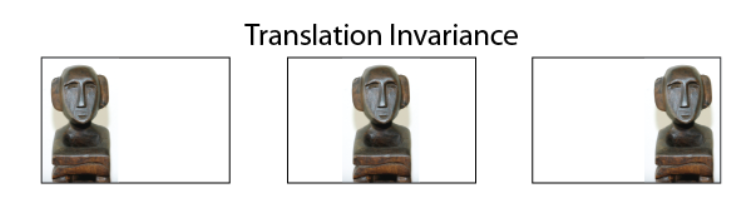
\includegraphics[width=0.8\textwidth]{img/translation_invariance.png}
    \caption{Las tres estatuas deben identificarse como iguales, aunque se ecuentren desplazadas.}
    \label{fig:invarianza_traslaciones}
\end{figure}

\medskip

\noindent A continuación veremos que el operador que hemos elegido sí cumple esta propiedad.

\begin{lema}
    El operador $\Phi(f)=|\widehat{f}|$ es invariante por traslaciones.
\end{lema}

\begin{proof}
    \noindent Para ello tenemos que ver que si definimos para cada $c \in \mathbb{R}^d$, la traslación $L_cf(x)=f(x-c)$ se tiene que :  
    
    $$\widehat{L_cf}(w)=\int_{\mathbb{R}^d}{L_cf(x) e^{-ixw} dx}=\int_{\mathbb{R}^d}{f(x-c)e^{-ixw}dx}$$
    
    \noindent Y realizando el cambio de variable $x-c=y$ se tendría que: 
    
    \begin{align*}
        \int_{\mathbb{R}^d}{f(x-c)e^{-ixw}dx} &= \int_{\mathbb{R}^d}{f(y)e^{-i(y+c)w}dy}= \\      &=\int_{\mathbb{R}^d}{f(y)e^{-iyw}e^{-icw}dy}= \\ &=\int_{\mathbb{R}^d}=e^{-icw}\int_{\mathbb{R}^d}{f(y)e^{-iyw}dy}=e^{-icw}\widehat{f}(w)
    \end{align*}
    
    \noindent Por lo que se tiene que $|\widehat{L_cf}(w)|=|e^{-icw}| |\widehat{f}(w)|=|\widehat{f}(w)|$ y entonces $\Phi(f)=|\widehat{f}|$ es invariante a traslaciones. \qedhere
\end{proof}

\medskip
    
\noindent Sin embargo, la invaianza por traslaciones no es suficiente, necesitamos también que nuestro operador sea invariante frente a pequeñas deformaciones (difeomorfismos). Este hecho es de vital importancia en el contexto del procesamiento de imágenes y la visión por computador, pues nos permite caracterizar objetos presentes en imágen incluso si estos se ven afectados por pequeñas deformaciones.

\medskip

\noindent Empezamos así definiendo qué es un difeomorfismo: 

\begin{figure}[!h]
    \centering
    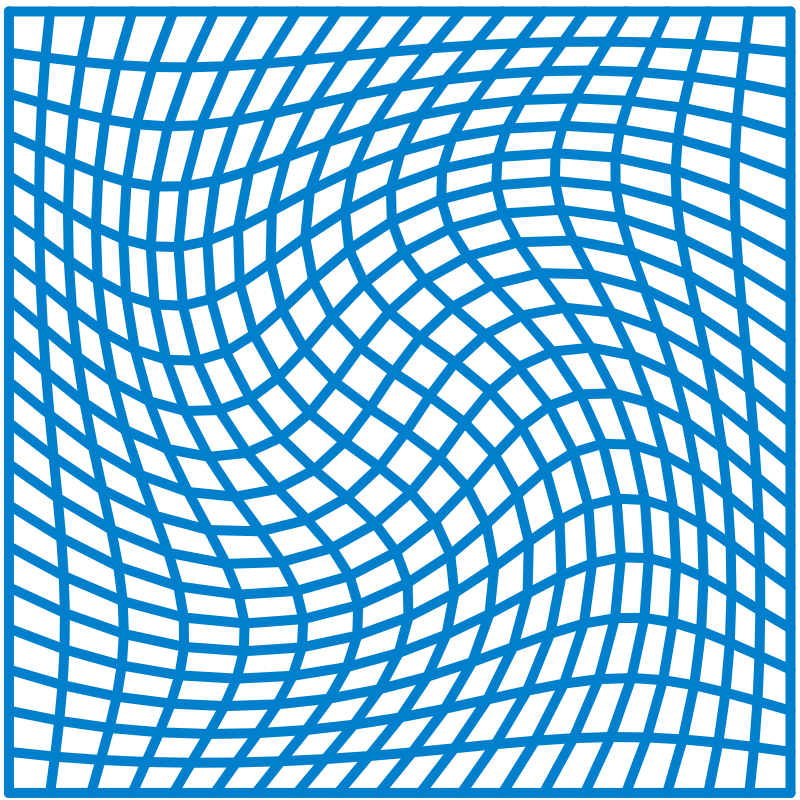
\includegraphics[width=0.5\textwidth]{img/Diffeomorphism.png}
    \caption{Acción de un difeomorfismo en una rejilla.}
    \label{fig:difeomorfismo}
\end{figure}

\begin{figure}[!h]
    \centering
    
\includegraphics[width=0.8\textwidth]{img/5_deformado.png}
    \caption{Todas las imágenes deberían clasificarse como 5, pese a las deformaciones.}
    \label{fig:deformaciones_5}
\end{figure}

\begin{figure}[!h]
    \centering
    
\includegraphics[width=0.5\textwidth]{img/1_excesivamente_deformado.png}
    \caption{Deformación excesiva que permite confundir el 1 con el 2 cuando se le aplica el difeomorfismo.}
    \label{fig:deformaciones_1}
\end{figure}

\begin{definicion}
    Una función diferenciable $f: X \rightarrow \Omega$ dónde $X$ y $\Omega$ son variedades, es un \entrecomillado{Difeomorfismo} si $f$ es una biyección y su inversa $f^{-1}:\Omega \rightarrow X$ es también diferenciable. 
\end{definicion}

\noindent Por otro lado, vamos a necesitar definir una distancia entre $\mathbb{1}$ y $\mathbb{1}-\tau$ para la condición de Lipschitz y garantizar la estabilidad bajo la acción de difeomorfismos:

\begin{definicion}
    La topología débil de los difeomorfismos de $C^2$ define una distancia entre $\mathbb{1}-\tau$ y $\mathbb{1}$ en cualquier subconjunto compacto $\Omega \in  \mathbb{R}^d$ mediante: 
    
    $$d_\Omega(\mathbb{1},\mathbb{1}-\tau) = \sup_{x \in \Omega} |\tau (x)| + \sup_{x \in \Omega} |\nabla \tau (x)| + \sup_{x \in \Omega}|H \tau (x)|$$
\end{definicion}

\noindent Dónde $|\tau(x)|$ es la norma euclídea en $\mathbb{R}^d$, $|\nabla \tau (x)|$ el supremo de la matriz $\nabla \tau (x)$ y $|H \tau (x)|$ el supremo de la norma del tensor Hessiano. Además se define $||\tau||_{\infty}\coloneqq \sup_{x\in\mathbb{R}^d} |\tau(x)|$.

\medskip 

\noindent De esta forma, un operador $\Phi(f)$ diremos que es estable frente a deformaciones si su norma euclídea $\left|\left| \Phi(f) - \Phi(L_\tau f) \right| \right|$ (con $L_{\tau} f(x)=f(x-\tau(x))$ definiendo la acción del difeomorfismo $\mathbb{1}-\tau$ en $f$) es \entrecomillado{pequeña} cuando la deformación se mide por $d_\Omega(\mathbb{1},\mathbb{1}-\tau)$. En otras palabras: 

\begin{definicion}
    Un Operador $\Phi$ invariante por traslaciones  se dice \entrecomillado{Lipschitz-continuo} bajo la acción de difeomorfismos de $C^2$ si para cualquier compacto $\Omega \in \mathbb{R}^d$ existe una constante $c\in \mathbb{R}^d$ tal que para todo $f\in L^2(\mathbb{R}^d)$ con soporte en $\Omega$ y $\tau \in C^2(\mathbb{R}^d)$ se tiene
    
    $$\left|\left| \Phi(f) - \Phi(L_\tau f) \right| \right| \leq c ||f|| (||\nabla \tau ||_{\infty} + ||H\tau||_\infty)$$
    
    con  $|| \nabla \tau ||_\infty + ||H \tau ||_\infty < 1$ para asegurarnos de que la deformación sea invertible \cite{doi:10.1137/S0036141002404838}.
\end{definicion}

\noindent Como podemos comprobar, la cota superior no depende de $||\tau(x)||_\infty$ ya que hemos supuesto que $\Phi$ es invariante por traslaciones. 

\noindent Sin embargo, esta propiedad no la verifica el módulo de la Transformada de Fourier, como podemos ver a continuación:

\begin{lema} \label{lemma:TF_inestable_difeomorfismos}
El módulo de la Transformada de Fourier no es estable frente a pequeñas deformaciones y no es \entrecomillado{Lipschitz-continuo}.
\end{lema}

\begin{proof}
\noindent Vamos a considerar la función $\tau(x)\coloneqq \epsilon x$ con $0 < \epsilon << 1$. De esta forma $||\nabla \tau (x) ||_\infty = \epsilon$ y $||H\tau(x)||_\infty=0$ con esto, la condición de Lipschitz debería ser

$$\left|\left| \; |\widehat{f}| -|\widehat{L_\tau f}| \; \right|\right| \leq c ||f|| (||\nabla \tau ||_{\infty} + ||H\tau||_\infty) \leq c ||f|| \epsilon$$

\noindent Si suponemos que $f(x)=e^{i\xi x} \Theta(x)$ el escalado por medio de $\tau$ produce que la frecuencia $\xi$ se traslade de $\xi$ a $(1-\epsilon)\xi$, si suponemos que $\Theta$ además es regular con decrecimiento rápido, se tiene que:

$$\left|\left| |\widehat{L_\tau f}|-|\widehat{f}| \right|\right| \sim |s| |\xi| ||\Theta|| = ||\nabla \tau||_\infty |\xi| ||f||.$$

\noindent Y como $|\xi|$ puede ser arbitrariamente grande, $\Phi(f)=|\widehat{f}|$ no satisface la continuidad de Lipschitz cuando se alcanzan altas frecuencias.
\end{proof}
    
\medskip

\noindent Por esto, lo que haremos será reemplazar las ondas sinusoidales de la transformada de Fourier por funciones localizadas con un soporte mayor en altas frecuencias que nos permitan evitar estas complicaciones, que tendrán un mejor rendimiento en nuestro propósito. Estas funciones se denominan \textbf{ondeletas}. 

\medskip

\subsubsection{Alternativa: Las ondeletas}

\noindent Las ondeletas \cite{MallatWavelets} son pequeñas ondas estables bajo la acción de deformaciones, al contrario que las ondas sinusoidales de Fourier. Definiremos la transformada de ondeletas y veremos que calcula, mediante convoluciones con bases de ondeletas, coeficientes que cumplirán con los requisitos que pedíamos para construir el operador del propagador de dispersión.

\medskip

\noindent Al contrario que las bases de Fourier, las bases de ondeletas definen  representaciones dispersas de señales regulares a trozos, que podrían incluir transiciones y singularidades. En las imágenes, los mayores coeficientes de las ondeletas se localizan en el entorno de las esquinas y en las texturas irregulares.

\medskip

\noindent A modo de ejemplo, vamos a ver la base de Haar, un ejemplo que aunque no sea el que utilicemos para construir nuestro propagador de dispersión, puede ayudar a entender mejor la filosofía de las ondeletas. Se construye a partir de la siguiente función: 

$$ \psi(t)= \begin{cases} 
      1 & 0\leq t < 1/2 \\
      -1 & 1/2\leq t < 1 \\
      0 & \; en \; otro \; caso
   \end{cases}$$

\begin{figure}[!h]
  \centering
  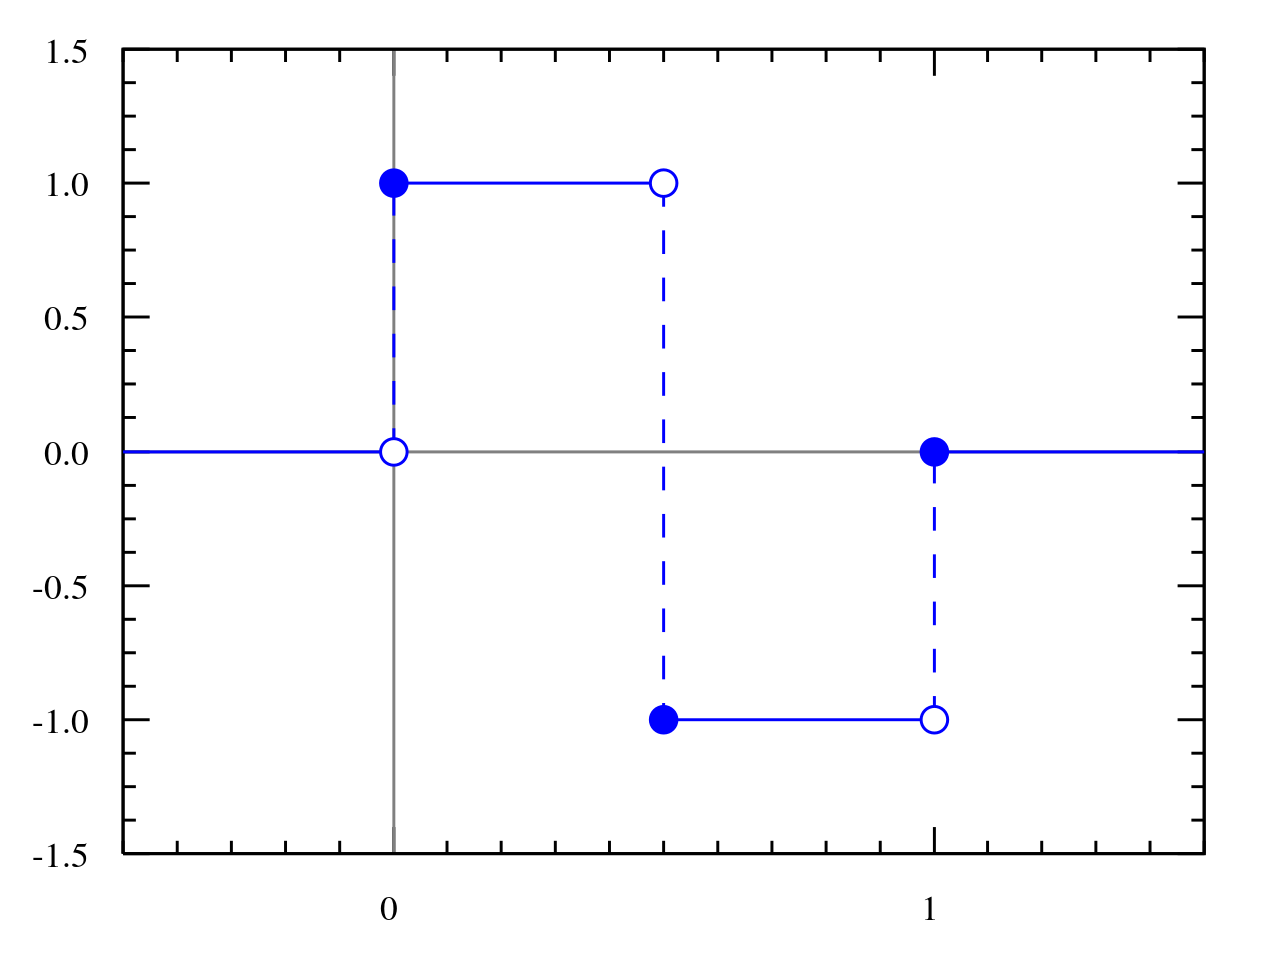
\includegraphics[width=0.5\textwidth]{img/Haar_wavelet.png}
  \caption{Representación gráfica de la ondeleta de Haar.}
  \label{fig:Ondeleta_de_Haar}
\end{figure}

\noindent A esta ondeleta la denominamos \textbf{ondeleta Madre}, pues a partir de ella, podemos generar la siguiente base ortonormal:

\medskip

$$\left \lbrace \psi_{j,n}(t)= \frac{1}{\sqrt{2^j}} \psi\left(\frac{t-2^jn}{2^j}\right) \right\rbrace_{(j,n) \in \mathbb{Z}^2}$$

\noindent del espacio $L^2(\mathbb{R})$ de señales con energía finita, si recordamos, en este espacio la norma se define como: 

\begin{definicion}
  $$||f||^2=\int_{-\infty}^{+\infty} |f(t)|^2 dt < +\infty$$
\end{definicion}

\noindent Así, cualquier señal $f$ de energía finita puede ser representada por los coeficientes que se obtienen mediante el producto interno en $L^2(\mathbb{R})$ con la base anterior: 

$$\langle f,\psi_{j,n} \rangle =\int_{-\infty}^{+\infty} f(t) \psi_{j,n} (t) dt  $$

\noindent y puede recuperarse sumando en su base ortonormal:

$$f=\sum_{j=-\infty}^{+\infty}\sum_{n=-\infty}^{+\infty}  \langle f,\psi_{j,n} \rangle \psi_{j,n} $$

\noindent Esto nos permite (igual que pasaba con el módulo de la Transformada de Fourier) trabajar en un dominio más sencillo que nos permite procesar la información con mayor rapidez y posteriormente reconstruir la señal a partir de los coeficientes sin perder información. Algunas propiedades serían: 

\begin{itemize}
  \item Cada ondeleta $\psi_{j,n}$ tiene media $0$ en su soporte $[2^jn, 2^j(n+1)]$.
  \item Si $f$ es localmente regular y $2^j$ es pequeño, entonces es casi constante en su intervalo y su coeficiente de ondeleta $\langle f,\psi_{j,n} \rangle$ es prácticamente cero.
  \item los mayores coeficientes se localizan en los cambios bruscos de intensidad de señal, como pueden ser los bordes, las esquinas o las texturas en las imágenes.
\end{itemize}

\noindent Para el caso concreto de imágenes (ver por ejemplo sección 1.1 de \cite{MallatWavelets}), las bases de ondeletas ortonormales pueden construirse a partir de bases ortonormales en señales de una dimensión. Así, a partir de tres ondeletas $\psi^1(x)$, $\psi^2(x)$ y$\psi^3(x)$ con $x=(x_1,x_2)\in \mathbb{R}^2$, dilatadas por el factor $2^j$ y trasladadas por $2^jn$ con $n=(n1,n2)\in \mathbb{Z}^2$, se construye una base ortonormal para el espacio $L^2(\mathbb{R}^2)$: 
$$\left \lbrace \psi_{j,n}^k(x)= \frac{1}{\sqrt{2^j}} \psi^k\left(\frac{x-2^jn}{2^j}\right) \right \rbrace_{(j,n) \in \mathbb{Z}^2}$$

\medskip

\noindent El soporte de la ondeleta $\psi_{j,n}^k(x)$ es un cuadrado proporcional a la escala $2^j$. Las bases de ondeletas en dos dimensiones se discretizan para definir bases ortonormales de imágenes de N píxeles.


\noindent Del mismo modo que en una dimensión, los coeficientes de ondeletas $\langle f,\psi_{j,n}^k \rangle$ serán pequeños si $f(x)$ es regular, y serán grandes cerca de los cambios bruscos de frecuencias como en los bordes o esquinas de las imágenes, como podemos ver en \autoref{fig:ejemplo_haar}. Los filtros resaltan los bordes en tres direcciones, horizontal (derecha) vertical (abajo) y en diagonal (abajo derecha).

\begin{figure} [!h]
  \centering
  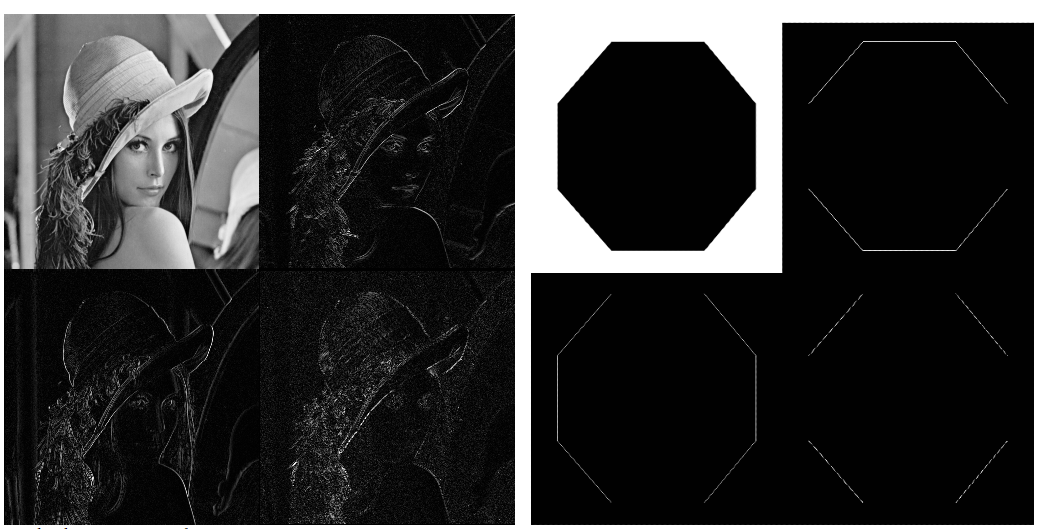
\includegraphics[width=0.8\textwidth]{img/ejemplos_haar_basis.png}
  \caption{Ejemplos de aplicar la base de Haar a dos imágenes \cite{HaarBasis}.}
  \label{fig:ejemplo_haar}
\end{figure}

\medskip 

\noindent Volviendo al propósito de definir el propagador de dispersión, la ondeleta madre que elijamos y la base ortogonal que forme se verán afectadas normalmente por escalados y rotaciones, por lo tanto definimos: 

\begin{definicion}
  Una ondeleta madre escalada por un factor $2^-j$ con $j \in \mathbb{Z}$ y rotada por $r \in G$ siendo $G$ el grupo finito de rotaciones, se escribe: 

  $$\psi_{2^j r}(x)=2^{dj} \psi(2^j r^{-1} x).$$
\end{definicion}


\medskip

\noindent Su transformada de Fourier es $\widehat{\psi_{2^j r}}(\omega)=\widehat{\psi}(2^j r^{-1} \omega)$.

\medskip

\noindent La transformada de dispersión que usaremos tendra una base de ondeletas generada por una ondeleta madre del tipo:

$$\psi(x)=e^{i\cdot \eta \cdot  x} \Theta(x)$$

\noindent Donde $\widehat{\Theta}(x)$ es una función real centrada en una bola de baja frecuencia en $x=0$, cuyo radio es del orden de $\pi$.

\medskip

\noindent Y como podemos ver:

$$(2.2) \;\;\; \widehat{\psi}(\omega)=\int_{\mathbb{R}^d}e^{i\cdot \eta \cdot  x} \Theta(x) e^{-i\omega x} dx=\int_{\mathbb{R}^d}\Theta(x) e^{ix(\omega-\eta)} dx=\widehat{\Theta}(\omega-\eta).$$

\medskip

\noindent Por lo tanto, $\widehat{\psi}(\omega)$ es real y centrada en una bola de mismo radio pero centrada en $\omega=\eta$ que tras el escalado y rotación: 
$$\widehat{\psi}_\lambda(\omega)= \widehat{\Theta} (\lambda^{-1}\omega-\eta),$$ 

\noindent donde $\lambda=2^jr \in 2^{\mathbb{Z}}\times G$. 

\noindent Por lo tanto $\widehat{\psi}_\lambda(\omega)$ recubre una bola centrada en $\lambda^{-1}\eta$ con radio proporcional a $|\lambda|=2^j$.
 
\medskip 

\subsubsection{La Transformada de Littlewood-Paley}

\noindent Una vez conocemos un poco más en profundidad las ondeletas y su foncionamiento, pasamos a presentar la \textbf{Transformada de ondeleta de Littlewood-Paley}, que es la que emplearemos para construir el propagador de dispersión.

\noindent Se trata de una representacion redundante que calcula convoluciones para todo $x \in \mathbb{R}^d$ sin realizar sub-muestreo: 

$$(2.4) \; \; \forall x \in  \mathbb{R}^d \;\; W[\lambda]f(x)= f \ast \psi_\lambda(x)=\int f(u)\psi_\lambda(x-u) du .$$

\noindent Dónde $\ast$ denota la operación de convolución. 

\medskip

\noindent Calculamos su transformada de Furier, para ello tendremos en cuenta el teorema de Convolución de la Transformada de Fourier, el cual dice: 

\begin{teorema} \label{Teorema::Convolucion}
 Sean $f$ y $g$ dos funciones integrables.

 Si 

 $$h(x)=(f\ast g)(x)=\int f(y)g(x-y) dy$$

 Entonces: 

 $$\widehat{h}(\omega)=\widehat{f}(\omega) \widehat{g}(\omega)$$

 y 

 $$h(x)=(f \ast g)(x)= \int \widehat{f}(\omega) \widehat{g}(\omega) e^{-i\Omega x} d\omega$$
 
\end{teorema}

De esta manera, se tiene que: 

$$\widehat{W[\lambda]f(\omega)}=\widehat{f}(\omega)\widehat{\psi_\lambda}(\omega)=\widehat{f}(\omega)\widehat{\psi}(\lambda^{-1}\omega).$$

\noindent Además, teniendo en cuenta la propiedad que nos dice que si la función $f$ es real, entonces su transformada coincide con el conjugado complejo $\widehat{f}(-\omega)=\overline{\widehat{f}(\omega)}$ podemos ver que: 

\begin{itemize}
  \item si $\widehat{\psi}(\omega)$ y $f$ son reales entonces $W[-\lambda]f= \overline{W[\lambda]f}$, utilizando la misma propiedad de antes.Además, si denotamos por $G^{+}$ al cociente de G con $\lbrace-\mathbb{1},\mathbb{1}\rbrace$, conjunto en el cual las dos rotaciones $r$ y $-r$ son equivalentes, sería suficiente calcular $W[2^jr]f$ para las rotaciones "positivas" de $G^{+}$
  \item En cambio, si $f$ fuese compleja, entonces $W[2^jr]f$ tendría que calcularse para todo $r \in G$
\end{itemize}

\medskip
 
\noindent La transformada de Littlewood-Paley a una cierta escala $2^J$ sólo mantiene las ondeletas de frecuencias $2^j>2^{-J}$ pues el resto de ondeletas de la base no tendrían soporte. De esta forma, las bajas frecuencias que no son cubiertas por estas ondeletas vienen dadas por un promedio en el dominio proporcional a $2^J$:

$$(2.5) \; \; A_Jf=f \ast \phi_ {2^J} \; \; con \; \phi_ {2^J}(x)=2^{-dJ} \phi(2^{-J}x). $$
\medskip

\noindent Así, si $f$ fuese real, entonces la transformada de ondeleta tendría la siguiente expresión: 

$$W_J f=\lbrace A_Jf,(W[\lambda]f)_{\lambda \in \Lambda_J} \rbrace$$ 

\noindent Es decir, estaría formada por el promedio de todas las odeletas de la base que no tienen soporte a la escala fijada $2^J$, y el conjunto de coeficientes producidos al convolucionar cada elemento de la base con $2^j>2^{-J}$ con la señal $f$. Para denotar esto indexamos por $\Lambda_J=\lbrace \lambda=2^jr:\;r\in G^{+}, \; 2^j>2^{-J}\rbrace$. 

\medskip

\noindent Su norma sería: 

$$(2.6) \; \; ||W_Jf||^2=||A_Jf||^2+\sum_{\lambda \in \Lambda_j} ||W[\lambda]f||^2.$$

\medskip
 
\noindent Si $J=\infty$ entonces todas las ondeletas de la base obtendrían coeficientes no nulos y por lo tanto 
$$W_\infty f=\lbrace W[\lambda]f\rbrace_{\lambda \in \Lambda_\infty},$$ 

\noindent con $\Lambda_\infty=2^\mathbb{Z} \times G^{+}$. 

\noindent Su norma en este caso sería 

$$||W_\infty f||^2=\sum_{\lambda \in \Lambda_\infty} ||W[\lambda]f||^2.$$

\noindent En el caso en que $f$ sea compleja, se incluyen todas las rotaciones $W_Jf=\lbrace A_J f,(W[\lambda]f)_{-\lambda,\lambda \in \Lambda_J} \rbrace$ y $W_\infty f=\lbrace W[\lambda]f\rbrace_{-\lambda,\lambda \in \Lambda_\infty}$. 

\medskip

\noindent La siguiente proposición da una condición estándar de Littlewood-Paley para que $W_J$ sea unitario.

\begin{proposicion} \label{unitario}
 Para cualquier $J \in \mathbb{Z}$ o $J=\infty$, $W_J$ es unitario en el espacio de funciones reales o complejas de $L^2(\mathbb{R}^d)$ si y sólo si para casi todo $\omega \in \mathbb{R}^d$: 
 
    \begin{align*}
        (2.7) \; \; \beta \sum_{j=-\infty}^\infty \sum_{r \in G} |\widehat{\psi}(2^{-j}r^{-1}\omega)|^2=1 & \; \; y
        \;\;|\widehat{\phi}(\omega)|^2= \beta \sum_{j=-\infty}^0 \sum_{r\in G} |\widehat{\psi}(2^{-j}r^{-1}\omega)|^2,
    \end{align*}
 Dónde $\beta=1$ para funciones complejas y $\beta=\frac{1}{2}$ para funciones reales.
\end{proposicion}

\begin{proof}
\noindent Si $f$ es una función compleja, $\beta=1$, y vamos a demostrar que (2.7) es equivalente a : 

$$(2.8) \; \; \forall J \in \mathbb{Z} \; \; \; \left|\widehat{\phi}\left(2^J\omega\right)\right|^2 + \sum_{j>-J,r\in G}\left|\widehat{\psi}\left(2^{-j}r^{-1}\omega\right)\right|^2=1. $$

\noindent Para ello partimos de que si $\beta=1$ se tiene sustituyendo en (2.7) que: 
     \begin{align*}
        \sum_{j=-\infty}^\infty \sum_{r \in G} |\widehat{\psi}(2^{-j}r^{-1}\omega)|^2=1 & \; \; y
        \;\;|\widehat{\phi}(\omega)|^2= \sum_{j=-\infty}^0 \sum_{r\in G} |\widehat{\psi}(2^{-j}r^{-1}\omega)|^2.
    \end{align*}

\noindent Si ahora sumamos $\sum_{j=0}^{\infty} \sum_{r\in G} |\widehat{\psi}(2^{-j}r^{-1}\omega)|^2$ en el segundo término obtenemos: 

$$|\widehat{\phi}(\omega)|^2 + \sum_{j=0}^{\infty} \sum_{r\in G} |\widehat{\psi}(2^{-j}r^{-1}\omega)|^2=1.$$

\noindent Por otro lado si vamos a la expresión a la que queremos llegar se tiene que: 

$$\forall J \in \mathbb{Z} \; \; \; \left|\widehat{\phi}\left(2^J\omega\right)\right|^2 + \sum_{j>-J,r\in G}\left|\widehat{\psi}\left(2^{-j}r^{-1}\omega\right)\right|^2=1 \iff \forall J \in \mathbb{Z} \; \; \; \left|\widehat{\phi}\left(2^J\omega\right)\right|^2=\sum_{j=-\infty}^{-J} \sum_{r\in G} |\widehat{\psi}(2^{-j}r^{-1}\omega)|^2.$$

\noindent Con lo que si demostramos esto último tendríamos que (2.7) y (2.8) son equivalentes para el caso $\beta=1$. 


     \begin{align*}
        \left|\widehat{\phi}\left(2^J\omega\right)\right|^2 & =\sum_{j=-\infty}^{0} \sum_{r\in G} |\widehat{\psi}(2^{-j}r^{-1}2^J\omega)|^2 \\
        & = \sum_{j=-\infty}^{0} \sum_{r\in G} |\widehat{\psi}(2^{J-j}r^{-1}\omega)|^2  \\
        & =\sum_{j=-\infty}^{-J} \sum_{r\in G} |\widehat{\psi}(2^{-j}r^{-1}\omega)|^2  
    \end{align*}
    
\noindent con lo que queda demostrado que (2.7) y (2.8) son equivalentes. Teniendo en cuenta que $\widehat{W\left[2^jr\right]f}(\omega)=\widehat{f}(\omega)\widehat{\psi}_{s^jr}(\omega)$, multiplicando (2.8) por $|\widehat{f}(\omega)|^2$ obtenemos: 

$$\forall J \in \mathbb{Z} \; \; \; \left|\widehat{\phi}\left(2^J\omega\right)\right|^2 \left|\widehat{f}(\omega)\right|^2 + \sum_{j>-J,r\in G}\left|\widehat{f}(\omega)\right|^2\left|\widehat{\psi}\left(2^{-j}r^{-1}\omega\right)\right|^2=\left|\widehat{f}(\omega)\right|^2.$$

\noindent Si ahora integramos en ambos miembros en $\mathbb{R}^d$ obtenemos: 

     \begin{align*}
        \int_{\mathbb{R}^d}\left(\left|\widehat{\phi}\left(2^J\omega\right)\right|^2 \left|\widehat{f}(\omega)\right|^2 + \sum_{j>-J,r\in G}\left|\widehat{f}(\omega)\right|^2\left|\widehat{\psi}\left(2^{-j}r^{-1}\omega\right)\right|^2 \right) d\omega=\int_{\mathbb{R}^d}\left|\widehat{f}(\omega)\right|^2 d\omega.
    \end{align*}
    
\noindent Recordamos la fórmula de Plancharel en el caso de $\mathbb{R}^d$: 

$$\int_{\mathbb{R}^d} \left|f(x)\right|^2 dx= \int_{\mathbb{R}^d}\left|\widehat{f}(\omega)\right|^2 d\omega.$$

\noindent Si la aplicamos a la expresión anterior se obtiene:

$$\int_{\mathbb{R}^d}\left(\left|\phi\left(2^J\omega\right)\right|^2 \left|f(\omega)\right|^2 + \sum_{j>-J,r\in G}\left|f(\omega)\right|^2\left|\psi\left(2^{-j}r^{-1}\omega\right)\right|^2 \right) d\omega=\int_{\mathbb{R}^d}\left|f(\omega)\right|^2 d\omega.$$

\noindent Si ahora recordamos la expresión (2.6), tenemos que la expresión anterior equivale a:

$$||A_Jf||^2+\sum_{\lambda \in \Lambda_j} ||W[\lambda]f||^2=||W_J f||^2=||f||^2,$$

\noindent que es válido para todo $J$ y en particular también cuando $J=\infty$.

\medskip

\noindent Recíprocamente, si tenemos que $||W_J f||^2=||f||^2$ entonces (2.8) se verifica para casi todo $\omega$. De no ser así podríamos contruir una función $f$ no nula cuya transformada de fourier $\widehat{f}$ tuviera soporte en el dominio de $\omega$ dónde (2.8) no fuera válido, y en estos casos al aplicar la fórmula de Plancherel se verificaría que $||W_J f||^2 \neq ||f||^2$ contradiciendo la hipótesis. Y como la expresión (2.8) era equivalente a la que nos daba el teorema tenemos demostrado el resultado para el caso en que $f$ sea compleja. 

\medskip

\noindent Si ahora $f$ es real entonces $|\widehat{f}(\omega)|=|\widehat{f}(-\omega)|$ lo que implica que $||W[2^jr]f||=||W[-2^jr]f||$. Por lo que $||W_J f||$ permanece constante si restringimos $r$ a $G^+$ y multiplicando $\psi$ por $\sqrt{2}$ se obtiene la condición (2.7) con $\beta=\frac{1}{2}$. \qedhere

\end{proof}

\medskip


\subsubsection{Convenios para futuras secciones}

\noindent LLegados a este punto, ya tenemos la transformada de ondeletas que vamos a utilizar para la construcción del PD, ahora vamos a establecer algunas características que impondremos a los distintos elementos que la componen y que usaremos de ahora en adelante: 

\begin{itemize}
    \item $\widehat{\psi}$ es una función real que satisface la condición (2.7). Lo que implica que $\widehat{\psi}(0)=\int \psi(x)dx=0$ y $|\widehat{\phi}(r\omega)|=|\widehat{\phi}(\omega)| \;\; \forall r\in G$.
    \item $\widehat{\phi}(\omega)$ es real y simétrica, por lo que $\phi$ también lo será y $\phi(rx)=\phi(x) \;\; \forall r \in G$. 
    \item Suponemos que $\phi$ y $\psi$ son dos veces diferenciables y su decrecimineto así como el de sus derivadas de primer y segundo orden es $O((1+|x|)^{-d-2})$.
\end{itemize}

\medskip

\noindent Un cambio de variable en la integral de la transformada de ondeleta nos muestra que si $f$ se escala y rota, $2^lg \circ f=f(2^lgx)$ con $2^lg \in 2^{\mathbb{Z}} \times G$, entonces la transformada de ondeleta se escala y rota de acuerdo a: 

$$(2.9) \;\;\; W[\lambda](2^lg\circ f)=2^lg \circ W[2^{-l}g\lambda]f.$$

\medskip

\noindent Como $\phi$ es invariante a traslaciones en $G$, podemos comprobar que $A_J$ conmuta con las rotaciones de $G$: $A_J(g\circ f)=g\circ A_J f \;\; \forall g \in G$. 

\subsection{El operador de dispersión sobre un camino ordenado}

%Esto debería intentar explicarlo mejor?
\noindent La transformada de Littlewood-Paley definida anteriormente es Lipschitz-conitnua bajo la acción de difeomorfismos, porque las ondeletas son funciones regulares y localizadas. Sin embargo, todavía no es invariante a traslaciones y $W[\lambda]f=f\ast\psi_\lambda$ se traslada cuando lo hace $f$.

\noindent Por eso el mayor reto es conseguir calcular coeficientes que sean invariantes a traslaciones, que permanezcan estables bajo la acción de difeomorfismos y que retengan la información en altas frecuencias que proporcionan las ondeletas, reuniendo todas estas características tendríamos el operador que necesitamos para la construcción del PD. 

\medskip 

\noindent Los coeficientes invariantes por traslaciones los obtendremos gracias a la acción de un operador no lineal aplicando el siguiente lema: 

%No se si perder tiempo en buscar la dem
\begin{lema} \label{lema:Invarianza_traslaciones_integral}
  Si $U[\lambda]$ es un operador definido en $L^2(\mathbb{R}^d)$, no necesariamente lineal pero que conmuta con traslaciones, entonces $\int_{\mathbb{R}^d} U[\lambda]f(x)dx$ es invariante a traslaciones si es finito.
\end{lema}

\begin{proof}
  Sea $f \in L^2(\mathbb{R}^d)$, $c \in \mathbb{R}^d$ y $L_cf(x)=f(x-c)$ una traslación de $f$, como $U[\lambda]f$ conmuta con traslaciones se tiene que: 
  \begin{align*}
    U[\lambda]L_cf(x)&=U(f(x-c)) \\
    &=U(f)(x-c) \\
    &=L_cU[\lambda]f(x)\\
  \end{align*}

  \noindent Vamos a comprobar ahora que si $\int_{\mathbb{R}^d} U[\lambda]f(x)dx$ es finito, entonces la integral es invariante a traslaciones. En otras palabras, queremos comprobar que : 

  $$\int_{\mathbb{R}^d} U[\lambda]L_cf(x)dx=\int_{\mathbb{R}^d} U[\lambda]f(x)dx$$

  Para ello, si tenemos en cuenta la conmutatividad del operador $U[\lambda]$ se tiene que 
  
  \begin{align*}
    \int_{\mathbb{R}^d} U[\lambda]L_cf(x)dx &= \int_{\mathbb{R}^d} U[\lambda](f(x-c))dx \\
    &= \int_{\mathbb{R}^d} U[\lambda](f)(x-c)dx. \\
  \end{align*}

  \noindent Y tras esto basta tener en cuenta el cambio de variable $y=x-c$ que tiene Jacobiano $J=1$ y se tendría que en la expresión anterior
  \begin{align*}
    \int_{\mathbb{R}^d} U[\lambda](f)(x-c)dx = \int_{\mathbb{R}^d} U[\lambda](f)(y)dy .\\
  \end{align*}
  
  \noindent Por lo que la integral es invariante por traslaciones.
\end{proof}

\noindent En nuestro caso $W[\lambda]f=f\ast\psi_\lambda$ es un ejemplo trivial de este lema, pues se trata de un operador que conmuta con traslaciones y $\int_{\mathbb{R}^d} f \ast \psi(x) dx=0$ porque $\int_{\mathbb{R}^d} \psi(x)dx=0$.

\medskip

\noindent Esto nos enseña, que para obtener un operador invariante por traslaciones y no trivial $U[\lambda]f$, es necesario componer $W[\lambda]$ con un operador extra $M[\lambda]$ que sea \entrecomillado{no lineal}, y que se conoce como "demodulación", que transforma $W[\lambda]f$ en una función de menor frecuencia con integral distinta de cero. Además, la elección de $M[\lambda]$ debe preservar la Lipschitz-continuidad bajo la acción de difeomorfismos.    
En resumen, queremos un operador no lineal que produzca coeficientes invariantes por traslaciones no triviales y que además conserve la Lipschitz-continuidad.


\medskip

\noindent Vamos a poner un ejemplo para entender mejor lo que se ha comentado anteriormente: 

\subsubsection{Ejemplo para obtener coeficientes invariantes por traslaciones}

\noindent Si la \textbf{ondeleta madre} fuese $\psi(x)=e^{i\eta x}\Theta(x)$, entonces los elementos de la base tendrían la forma $\psi_\lambda(x)=e^{i\lambda\eta x}\Theta_\lambda(x)$, y por lo tanto 

\begin{align*}
  W[\lambda]f(x) &= f \ast \phi_\lambda (x) \\
  &= f \ast e^{i\lambda\eta x}\Theta_\lambda(x) \\
  &=e^{i\lambda\eta x}(e^{-i\lambda\eta x}f(x) \ast \Theta_\lambda(x)) \\
  &=e^{i\lambda\eta x}(f^\lambda \ast \Theta_\lambda(x)),\\
\end{align*}

\noindent con $f^\lambda(x)=e^{-i\lambda\eta x}f(x)$.

\medskip

\noindent En este caso, se podría obtener un operador invariante por traslaciones si se cancela el término de modulación $e^{i\lambda\eta x}$ con una función $M[\lambda]$ pertinente. Por ejemplo: 

$$(2.12) \;\;\; M[\lambda]h(x)=e^{-i\lambda\eta x} e^{-i \Phi(\widehat{h}(\lambda\eta))}h(x).$$

\noindent Dónde $\Phi(\widehat{h}(\lambda\eta))$ es la fase compleja de $\widehat{h}(\lambda\eta)$. Este registro de fase no lineal garantiza que $M[\lambda]$ conmuta con las traslaciones, ya que: 


\begin{align*}
  \int_{\mathbb{R}^d} M[\lambda]W[\lambda] f(x) dx &= \int_{\mathbb{R}^d} e^{-i\lambda \eta} e^{-i \Phi (\widehat{W[\lambda\eta]f})} \left( e^{i\lambda\eta x} \left( e^{-i\lambda\eta x} f \ast \Theta_\lambda (x)\right)\right) dx \\
  &= e^{-i \Phi (\widehat{f}(\lambda\eta)\widehat{\psi_\lambda}(\lambda\eta))} \int_{\mathbb{R}^d} e^{-i\lambda\eta x} f \ast \Theta_\lambda (x) dx \\
  &=e^{-i \Phi (\widehat{f}(\lambda\eta)\widehat{\psi_\lambda}(\lambda\eta))} \int_{\mathbb{R}^d}e^{-i\lambda\eta x} f(x) dx  \int_{\mathbb{R}^d}\Theta_\lambda (x) dx  \\
  &=e^{-i \Phi (\widehat{f}(\lambda\eta)\widehat{\psi_\lambda}(\lambda\eta))} \cdot \widehat{f}(\lambda\eta) \cdot  \widehat{\Theta_\lambda}(0)\\
  &=\left| \widehat{f}(\lambda\eta) \cdot  \widehat{\Theta_\lambda}(0) \right|^2 \\
  &=\left| \widehat{f}(\lambda\eta)\right|^2 \left| \widehat{\Theta_\lambda}(0) \right|^2  \\
  &=\left| \widehat{f}(\lambda\eta)\right|^2 \left| \widehat{\Theta}(0) \right|^2 
\end{align*}

\noindent que como podemos ver, la integral tiene un valor no trivial y por otra parte obtenemos el módulo de la transformada que como habíamos visto era invariante por traslaciones. No obstante, no utilizaremos este operador para nuestro propósito pues además de ser complejo no verifica la invarianza bajo la acción de difeomorfismos.

\subsubsection{El operador módulo.}

\noindent En nuestro caso, para preservar la Lipschitz-continuidad bajo la acción de difeomorfismos necesitamos que $M[\lambda]$ conmute con estos y que además sea no expansiva para garantizar la estabilidad en $L^2(\mathbb{R}^d)$. Se puede comprobar que entonces $M[\lambda]$ tiene que ser necesariamente un operador punto a punto \cite{JBrunaOperatorsCommutingDiff}, lo que significa que el operador $M[\lambda]h(x)$ que buscamos dependería únicamente del valor de $h$ en el punto $x$.

\medskip

\noindent Para obtener mejores propiedades vamos a imponer también que $||M[\lambda]h||=||h|| \; \; \forall h \in L^2(\mathbb{R}^d)$, lo que implica entonces que $|M[\lambda]h|=|h|$, ya que:  

\begin{align*}
  ||M[\lambda]h||=||h|| &\iff \left(\int_{\mathbb{R}^d} |M[\lambda]h (x)|^2 dx \right)^{\frac{1}{2}} =\left(\int_{\mathbb{R}^d} |h(x)|^2 dx \right)^{\frac{1}{2}} \\
  & \iff \int_{\mathbb{R}^d} |M[\lambda]h (x)|^2 dx=\int_{\mathbb{R}^d} |h(x)|^2 dx \\
  & \iff |M[\lambda]h (x)|^2=|h(x)|^2 \\
  & \iff |M[\lambda]h (x)|=|h(x)|
\end{align*}

\medskip

\noindent Para satisfacer todas las restricciones, utilizaremos el operador $M[\lambda]h=|h|$, que además elimina todas las variaciones de fase \cite{bruna2013invariant}. Se obtiene entonces de $(2.11)$ que este módulo transforma $W[\lambda]f$ en una señal de menor frecuencia que la original:

$$M[\lambda]W[\lambda]f=|W[\lambda]f|=|f^\lambda \ast \Theta_\lambda|.$$

%Ejemplo:
\noindent Vamos a visualizar con un ejemplo cómo al interferir dos señales con este operador, la frecuencia resultante es menor que cada una de las originales. 

\medskip

\noindent Por ejemplo, si 

$$f(x)=\cos(\xi_1 x)+a\cos(\xi_2 x)$$

\noindent dónde $\xi_1$ y $\xi_2$ están en la banda de frecuencia cubierta por $\widehat{\psi}_\lambda$, entonces al aplicar el operador módulo: 

$$|f \ast \psi_\lambda (x) |=2^{-1} |\widehat{\psi}_\lambda(\xi_1)+a\widehat{\psi}_\lambda(\xi_2)e^{i(\xi_2-\xi_1)x}|$$

\noindent que oscila entre la frecuencia de interferencias $|\xi_2-\xi_1|$, que como vemos es menor que $|\xi_1|$ y $|\xi_2|$.

\medskip

\noindent De esta manera, por la forma en que hemos construido el operador $U[\lambda] f$ la integración de $\int_{\mathbb{R}^d}U[\lambda]f(x) dx= \int_{\mathbb{R}^d} | f \ast \psi_\lambda(x)|dx$ es invariante por traslaciones pero elimina todas las altas frecuencias de $|f \ast \psi_\lambda(x)|$. Para recuperarlas, el PD calcula los coeficientes de ondeletas para cada $U[\lambda]f$ que son $\lbrace U[\lambda]f \ast \psi_{\lambda'}\rbrace_{\lambda'}$. De nuevo, los coeficientes invariantes a traslaciones se obtienen con el módulo $U[\lambda']U[\lambda]f=|U[\lambda]f \ast \psi_{\lambda'}|$ y después integrando $\int_{\mathbb{R}^d} U[\lambda']U[\lambda]f(x) dx$. 

\medskip

\noindent Veamos esto con el mismo ejemplo de antes $f(x)=\cos(\xi_1 x)+a\cos(\xi_2 x)$ pero con $a<1$. Si $|\xi_2-\xi_1| << |\lambda|$ con $|\xi_2 - \xi_1|$ en el soporte de $\widehat{\psi}_{\lambda'}$, entonces $U[\lambda']U[\lambda]f$ es proporcional a $a\cdot |\psi_\lambda(\xi_1)|\cdot |\psi_{\lambda'}(|\xi_2-\xi_1|)|$. La segunda ondeleta $\widehat{\psi}_{\lambda'}$ captura las interferencias creadas por el módulo, entre la frecuencia de las componentes de f y el soporte de $\widehat{\psi_\lambda}$.

\medskip

\noindent A continuación introducimos el PD que extiende estas descomposiciones.

\medskip

\begin{definicion}
Una secuencia ordenada $p=(\lambda_1,\lambda_2, ... , \lambda_m)$ con $\lambda_k \in \Lambda_\infty=2^{\mathbb{Z}} \times G^{+} $ se denomina \textbf{camino}. Al camino vacío se le denota por $p=\emptyset$. 
\end{definicion}


\begin{definicion}
Un PD es un producto de operadores de la forma $U[\lambda]f=M[\lambda]W[\lambda]f=|f \ast \psi_\lambda|=\left | \int_{\mathbb{R}^d} f(u)\psi_\lambda(x-u) du \right|$ para $f \in L^2(\mathbb{R}^d)$ no conmuntativos por un camino ordenado:

$$(2.13) \;\;\; U[p]f=U[\lambda_m]...U[\lambda_2]U[\lambda_1],$$

con $U[\emptyset]=Id$
\end{definicion}

\noindent El operador $U[p]$ está bien definido en $L^2(\mathbb{R}^d)$ porque $\left|\left| U[\lambda]f \right|\right| = ||f|| \leq ||\psi_\lambda||_1 ||f||$ para todo $\lambda \in \Lambda_\infty$. 

\noindent El PD es por tanto una cascada de convoluciones y módulos: 

$$(2.14) \;\;\; \left| |f \ast \psi_{\lambda_1} | \ast \psi_{\lambda_2} | ... | \ast \psi_{\lambda_m} \right|$$

\medskip

\noindent Cada $U[\lambda]$ filtra la frecuencia del componente en la banda cubierta por $\widehat{\psi}_\lambda$ y lo mapea en un espacio de frecuencias menores con la operación módulo.

\subsubsection{Propiedades de un camino de frecuencias.}

\noindent A continuación vamos a probar ciertas propiedades que tienen los caminos de frecuencias tal y como los hemos descrito anteriormente. Para ello empezamos con algunas definiciones que serán de utilidad:

\begin{definicion}
Escribimos la rotación y reescalo de un camino $p$ mediante $2^lg \in 2^\mathbb{Z}\times G$ como $2^lgp=(2^lg\lambda_1,2^lg\lambda_2,...,2^lg\lambda_m)$.
\end{definicion}

\begin{definicion}
La concatenación de dos caminos $p$ y $p'$ se denota por $p+p'=(\lambda_1,\lambda_2,...,\lambda_m,\lambda_1',\lambda_2',...,\lambda_{m'}')$. 

En el caso particular de $p+\lambda=(\lambda_1,\lambda_2,...,\lambda_m,\lambda)$
\end{definicion}

\noindent Con todo lo que sabemos sobre caminos, podemos probar la siguiente propiedad: 

\begin{proposicion} \label{proposicionSumaCaminos}
Sean $p, p'$ dos caminos, se tiene que :
$$U[p+p']=U[p']U[p]$$
\end{proposicion}

\begin{proof}
Como $p+p'=(\lambda_1,\lambda_2,...,\lambda_m,\lambda_1',\lambda_2',...,\lambda_{m'}')$ entonces siguiendo la definición de $U[p]$ se tiene que: 
$$U[p+p']=U[\lambda'_{m'}]...U[\lambda'_2]U[\lambda'_1]U[\lambda_{m}]...U[\lambda_2]U[\lambda_1]=U[p']U[p]$$ \qedhere
\end{proof}

\medskip

\noindent En la \autoref{ch:seccion12} veíamos que si $f$ era compleja, entonces su transformada de ondeletas era $ W_\infty=\lbrace W[\lambda]f \rbrace_{\lambda , -\lambda  \in \Lambda_{\infty} }$. Pero en este caso, gracias al módulo si $f$ es compleja, tras la iteración $U[\lambda_1]f=\left|W[\lambda_1]f\right|$ sería una función real, luego para las siguientes transfomadas de ondeletas sólo haría falta calcularlas para $\lambda_k \in \Lambda_\infty$. Por lo tanto para los propagadores de dispersión de funciones complejas se definen sobre caminos "positivos" $p=(\lambda_1,\lambda_2, ... , \lambda_m)$ y caminos "negativos" $-p=(-\lambda_1,\lambda_2, ... , \lambda_m)$.

\medskip

\noindent Sin embargo para simplificar cálculos, todos los resultados siguientes se haran sobre PD aplicados a funciones reales.

\subsubsection{Construcción del operador de dispersión.}

\noindent En este momento ya disponemos de un operador $U[\lambda] f$ que cumple todas las condiciones deseables , por lo que en esta sección vamos a ser capaces de llegar finalmente a la modelización matemática de una CNN.

\begin{definicion} \label{def:S_barra}
Sea $\mathcal{P}_\infty$ el conjunto de todos los caminos finitos. La transformada de dispersión de $f \in L^1(\mathbb{R}^d)$ se define para cualquier camino $p \in \mathcal{P}_\infty$ como:

$$(2.16) \; \; \; \overline{S}f(p)=\int_{\mathbb{R}^d}U[p]f(x)dx .$$
\end{definicion}

\medskip

\noindent El operador $\overline{S}f(p)$ es invariante a traslaciones de $f$, pues el operador $U[p]$ hemos visto que cumple las propiedades necesarias para que el valor de la integral sea finito y por lo tanto sea invariante por traslaciones, y transforma $f \in L^1(\mathbb{R}^d)$ en una función en el camino de frecuencias variable $p$.

\medskip

\noindent Esta defnición guarda muchas similitudes con la el módulo de la transformada de Fourier, pero en este caso la transformada es Lipschitz-continua bajo la acción de difeomorfismos, porque se calcula iterando en transformadas de ondeletas y módulos que, como hemos visto anteriormente, son estables. 

\medskip

\noindent No obstante, para problemas de clasificación, es mucho más frecuente calcular pequeños descriptores que sean invariantes por traslaciones frente a una escala predefinida $2^J$, manteniendo las frecuencias superiores a $2^J$, lo que nos permite ver esta variabilidad espacial. Esto se consigue convolucionando la transformada con una ventana escalada a la frecuencia deseada, en nuestro caso $\phi_{2^J}(x)=2^{-dJ}\phi(2^{-J}x)$. 

\begin{definicion}
Sea $J \in \mathbb{Z}$ y $\mathcal{P}_J$ el conjunto de caminos finitos $p=(\lambda_1,\lambda_2,...,\lambda_m)$ con $\lambda_k \in \Lambda_J$ y $|\lambda_k|=2^{jk}>2^{-J}$. Una ventana de transformada de dispersión se define para todo $p \in \mathcal{P}_J$ por

$$(2.20) \;\;\; S_J[p]f(x)=U[p]f \ast \phi_{2^J}(x)=\int_{\mathbb{R}^d}U[p]f(u)\phi_{2^J}(x-u)du.$$

$$(2.21) \;\;\; S_J[p]f(x)=\left| |f \ast \psi_{\lambda_1} | \ast \psi_{\lambda_2} | ... | \ast \psi_{\lambda_m} \right| \ast \phi_{2^J}(x).$$

Con $S_J[\emptyset] f= f \ast \phi_{2^j}$.
\end{definicion}


\noindent Esto define una familia infinita de funciones indexadas por $\mathcal{P}_J$, denotada por

$$S_J[\mathcal{P}_J]f \coloneqq \lbrace S_J[p]f \rbrace_{p\in\mathcal{P}_J}.$$

\medskip

\noindent Si nos fijamos, para cada camino $p$, $S_J[p]f(x)$ es una función que actúa sobre la ventana centrada en la posición $x$ cuyo tamaño serían intervalos de dimensión $2^J$.

\medskip

\noindent Para el caso de funciones complejas solo tendríamos que inculir en $\mathcal{P}_J$ los caminos negativos, y si $f$ es real $S_J[-p]=S_J[p]f$.
\noindent En la \autoref{ch:seccion13} se comprueba que para ondeletas apropiadas, $||f||^2=\sum_{p\in\mathcal{P}_J}\left|\left|S_J[p]f\right|\right|^2$. 

\medskip

\noindent Sin embargo, la energía de señal se concentra en un conjunto mucho más pequeño de caminos de frecuencias descendentes $p=(\lambda_k)_{k\leq m}$ en el cual $|\lambda_{k+1}| \leq |\lambda_k|$ como vimos en el ejemplo anterior. Esto ocurre porque como mencionamos antes, el propagador $U[\lambda]$ progresivamente lleva la energía de la señal a frecuencias cada vez menores, hasta que en cierto punto es nula.

\medskip

\noindent Veamos ahora la relación que guarda este propagador de ventana con el que se definió originalmente en \autoref{def:S_barra}. Como $\phi(x)$ es continua en $0$, si $f\in L^1 (\mathbb{R}^d)$ se tiene que su transformada de dispersión de ventana converge punto a punto a la transformada de dispersión cuando la escala $2^J$ tiende a $\infty$: 

\begin{align*}
    (2.21) \;\;\; \forall x \in \mathbb{R}^d \;\; \lim_{J \rightarrow \infty} 2^{dJ} S_J[p]f(x) &=\phi(0)\int_{\mathbb{R}^d}U[p]f(u) du \\
    &=\lim_{J \rightarrow \infty} 2^{dJ} U[p]f \ast \phi_{2^J}(x) \\
    &=\lim_{J \rightarrow \infty} 2^{dJ} \int_{\mathbb{R}^d} U[p]f(u)\phi_{2^J}(x-u) du \\
    &=\lim_{J \rightarrow \infty} 2^{dJ} \int_{\mathbb{R}^d} U[p]f(u) 2^{-dJ} \phi(2^{-J}(x-u)) du   \\
    &= \int_{\mathbb{R}^d} U[p]f \phi(0) du  \\
    &= \phi(0) \int_{\mathbb{R}^d} U[p]f du  \\
    &= \phi(0)\overline{Sf}(p).\\ 
\end{align*}

\subsection{Propagador de dispersión y conservación de la Norma} \label{ch:seccion13}


\subsubsection{Proceso de dispersión del propagador.}

\noindent Hasta ahora hemos probado que el propagador $S_J$ es no-expansivo y que preserva la norma de $L^2(\mathbb{R}^d)$. A partir de ahora denotamos por $S_J[\Omega] \coloneqq \lbrace S_J[p] \rbrace_{p\in\Omega}$ y $U[\Omega]\coloneqq \lbrace U[p] \rbrace_{p\in\Omega}$ a la familia de operadores indexados por el conjunto de caminos $\Omega \subset \mathcal{P}_\infty$.

\medskip

\noindent Un dispersor de ventanas $S_J$ puede calcularse iterando en el propagador de un paso definido anteriormente como: 

$$U_Jf=\lbrace A_Jf, (U[\lambda]f)_{\lambda\in\Lambda_J} \rbrace,$$

\noindent con $A_J=f\ast \phi_{2^J}$ y $U[\lambda]f=\left| f\ast \psi_\lambda \right|$. 

\medskip

\noindent Tras calcular $U_Jf$, aplicando de nuevo $U_J$ a cada coeficiente $U[\lambda]f$ se genera una familia infinita aún más grande de funciones. La descomposición se continúa iterando  por recursividad aplicando $U_J$ a cada $U[p]f$. 

\medskip

\noindent Teniendo en cuenta \autoref{proposicionSumaCaminos} se tiene que  $U[\lambda]U[p]=U[p+\lambda]$, y $A_JU[p]=S_J[p]$, esto dando lugar a : 

$$(2.22) \;\;\; U_JU[p]=\lbrace S_J[p]f,(U[p+\lambda]f)_{\lambda\in\Lambda_J}\rbrace.$$

\medskip

\noindent Podemos por tanto establecer el comportamiento de al transformada de dispersión según la longitud $m$ del camino que estamos empleando. Sea $\Lambda_J^m$ el conjunto de caminos de longitud $m$ con $\Lambda_J^0={\emptyset}$, entonces:

$$(2.23) \;\;\; U_J U[\Lambda_J^m]=\lbrace S_J[\Lambda_J^m]f,(U[\Lambda_J^{m+1}]f)_{\lambda\in\Lambda_J}\rbrace.$$

\noindent Del hecho de que $\mathcal{P}_J=\cup_{m\in \mathbb{N}}\Lambda_J^m$, uno puede calcular $S_J[\mathcal{P}_J]f$ a partir de $f=U[\emptyset]f$ iterativamente calculando $U_J U[\Lambda_J^m]f$ para $m$ tendiendo a $\infty$, tal y cómo se puede ver en la imagen \autoref{fig:scattering_propagator}. 

\begin{figure} [!h]
  \centering
  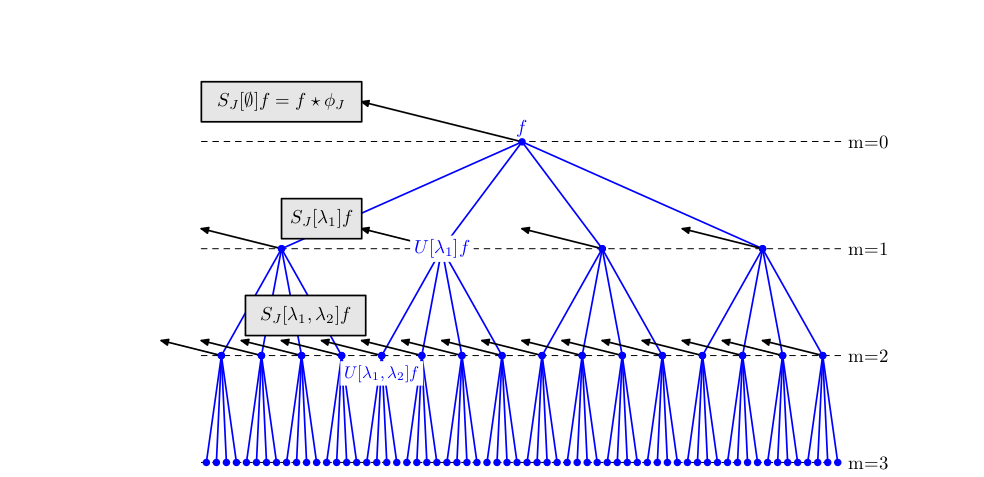
\includegraphics[width=0.8\textwidth]{img/ScatteringPropagator.png}
  \caption{Un PD $U_J$ aplicado a un punto de una señal $f(x)$ calcula $U[\lambda_1]f(x)=|f(x)\ast \psi_{\lambda_1}|$ y como salida a la capa $m=0$ se promedian los coeficientes que han dado $0$ (por tener $2^j<2^-j$) obteniendo como salida $S_J[\emptyset]f(x)=f(x)\ast \phi_{2^J}$ (como se puede ver en la flecha negra). Después se aplica de nuevo $U_J$ a cada coeficiente $U[\lambda_1]f(x)$ del paso anterior ($m=1$) $U[\lambda_1,\lambda2]f(x)$ obteniendo como salida $S_J[\lambda_1]f(x)=U[\lambda_1]f(x) \ast \phi_{2^J}$. Se repite este proceso de manera recursiva para cada coeficiente $U[p]f(x)$ y obteniendo como resultado $S_J[p]f(x)=U[p]f(x) \ast \phi_{2^J}$. }
  \label{fig:scattering_propagator}
\end{figure}


\subsubsection{Diferencias y similitudes con una CNN}


Las operaciones de la transformada de dispersión que hemos descrito siguen la estructura general de la red neuronal convolucional introducida por LeCun \cite{lecun2015deep}, pues se describen las redes convolucionales como una cascada de convoluciones (la transfomada de ondeletas $W[\lambda]$) y capas de "pooling" que usan funciones no lineales (el operador módulo $M[\lambda]$), las cuales se representan en este modelo como módulos de números complejos. También se puede considerar como un operador de \entrecomillado{pooling} la función $\phi_{2^J}$ que se emplea para agregar coeficientes y contruir un operador invariante.

\medskip

\noindent Las redes neuronales convolucionales han sido empleadas con mucho éxito en tareas de reconocimiento de objetos o personas y usan normalmente Kernels que no son predefinidos, sino que se aprenden mediante la técnica de back-propagation al entrenar la red, en cambio, en la modelización que se ha presentado las ondeletas que usamos son prefijadas y no se aprenden.

\medskip

\noindent Siguiendo con las similitudes entre ambos modelos, si $p$ es un camino de longitud $m$, entonces a $S_J[p] f(x)$ se le denomina coeficiente de orden $m$ a escala $2^J$, que en el caso de una CNN,equivaldría al tensor formado por los mapas de activación tras la convolución con el kernel de la capa $m$ de la red. 

\medskip


\subsubsection{Relación con herramientas clásicas de visión por computador}
\noindent Por otro lado, la modelización  con los algoritmos clásicos de visión por computador como \textbf{SIFT}  \cite{DistinctiveImageFeatures} para calcular puntos de interés en imágenes. Así, con la ondeletas apropiadas, los coeficientes de primer orden $S[\lambda_1] f$ serían equivalentes a los coeficientes del algoritmo. De hecho, en el artículo sobre el descriptor DAISY \cite{Daisy} se muestra cómo esos coeficientes son aproximados por $S_J[2^j r] f= | f \ast \psi_{2^j r} | \ast \phi_{2^J}(x)$, dónde $\psi_{2^j r}$ es la derivada parcial de una Gaussiana calculada en imagen de escala $2^j$ de mayor calidad, para 8 rotaciones distintas $r$. El filtro para promediar $\phi_{2^J}$ es un filtro Gaussiano escalado.


\subsubsection{Operador no expansivo.}

\noindent El propagador $U_Jf=\lbrace A_Jf, \left(\left| W[\lambda]f\right|\right)_{\lambda\in\Lambda_J} \rbrace$ es no expansivo, porque la transformada de ondas $W_J$ es unitaria pues cumple las hipótesis de la \autoref{unitario} y el módulo no es expansivo en el sentido de que $||a|-|b||\leq |a-b|$ para cualquier $(a,b)\in \mathbb{C}^2$. Esto es válido tanto si $f$ es real o compleja. Como consecuencia: 

\begin{align*} 
    ||U_J f-U_J h||^2 &= ||A_J f-A_J h||^2+\sum_{\lambda\in\Lambda_J} \left\| |W[\lambda]f|-|W[\lambda]h| \right\|^2 \\
    &\leq \left| \left| W_J f- W_J h \right| \right|^2 \leq ||f-h||^2 \;\;\; (2.24)
\end{align*}

\noindent Al ser $W_J$ unitaria, tomando la función nula $h=0$ y siguiendo el mismo razonamiento anterior, también se comprueba que $||U_J f||=||f||$ por lo que el operador $U_J$ preserva la norma.

\medskip

\noindent Para todo conjunto de caminos $\Omega$, las normas de $S_J[\Omega]f$ y $U[\Omega]f$ son: 

$$\left|\left| S_J[\Omega]f \right|\right|^2=\sum_{p\in\Omega} \left|\left| S_J[p]f\right|\right|^2 \;\; y \;\; \left|\left|U[\Omega]f\right|\right|^2=\sum_{p\in\Omega} \left|\left| U[p]f\right|\right|^2$$

\noindent Como $S_J[\mathcal{P}_J]$ itera en $U_J$, que es no expansivo, la siguiente proposición prueba que $S_J[\Omega]f$ es también no expansivo. 

\begin{proposicion}
La transformada de dispersión de ventana es no expansiva: 

$$(2.25) \;\;\; \forall (f,h)\in L^2(\mathbb{R}^d)^2 \;\; ||S_J[\mathcal{P}_J]f-S_J[\mathcal{P}_J]h|| \leq ||f-h||$$
\end{proposicion}

\begin{proof}
Como $U_J$ es no expansiva, partiendo de $(2.23)$ que nos dice: 
$$U_J U[\Lambda_J^m]=\lbrace S_J[\Lambda_J^m]f,(U[\Lambda_J^{m+1}]f)_{\lambda\in\Lambda_J}\rbrace,$$

se tiene que:

\begin{align*}
    ||U[\Lambda_J^m]f-U[\Lambda_J^m]h||^2 &\geq ||U_J U[\Lambda_J^m]f-U_J U[\Lambda_J^m]h||^2 \\
    & = ||S_J[\Lambda_J^m]f - S_J[\Lambda_J^m]h||^2 + ||U[\Lambda_J^{m+1}]f-U[\Lambda_J^{m+1}]h||^2.
\end{align*}

\medskip

\noindent Si ahora sumamos en $m$ cuando tiende a $\infty$ se obtiene que: 

\begin{align*}
  \sum_{m=0}^{\infty}||U[\Lambda_J^m]f-U[\Lambda_J^m]h||^2 &\geq \sum_{m=0}^{\infty} ||S_J[\Lambda_J^m]f - S_J[\Lambda_J^m]h||^2 + \sum_{m=0}^{\infty} ||U[\Lambda_J^{m+1}]f-U[\Lambda_J^{m+1}]h||^2,\\
\end{align*}

\noindent que equivale a:

\begin{align*}
  \sum_{m=0}^{\infty}||U[\Lambda_J^m]f-U[\Lambda_J^m]h||^2 - \sum_{m=0}^{\infty} ||U[\Lambda_J^{m+1}]f-U[\Lambda_J^{m+1}]h||^2 &\geq \sum_{m=0}^{\infty} ||S_J[\Lambda_J^m]f - S_J[\Lambda_J^m]h||^2\\
\end{align*}

\noindent Si ahora nos fijamos en el lado izquierdo de la desigualdad, se cancelan todos los términos salvo $m=0$, y teniendo en cuenta que $\Lambda^0_J=\emptyset$ queda: 

\begin{align*}
  \sum_{m=0}^{\infty}||U[\Lambda_J^0]f-U[\Lambda_J^0]h||^2 &= \sum_{m=0}^{\infty}||U[\emptyset]f-U[\emptyset]h||^2 = || f - h ||^2 \\
\end{align*}

\noindent Por otro lado, se tiene que

\begin{align*}
  \sum_{m=0}^{\infty} ||S_J[\Lambda_J^m]f - S_J[\Lambda_J^m]h||^2 = ||S_J[\mathcal{P}_J]f - S_J[\mathcal{P}_J]h||^2. \\
\end{align*}

\noindent Luego hemos probado que 

$$||S_J[\mathcal{P}_J]f - S_J[\mathcal{P}_J]h||^2 \leq || f - h ||^2$$

\noindent y por lo tanto que la transfomada de dispersión de ventana es no expansiva. \qedhere
\end{proof}

\subsubsection{Conservación de la norma.}

En la \autoref{ch:seccion12} se obtuvo que cada coeficiente $U[\lambda]f=|f \ast \psi_\lambda|$ capturaba la energía de frecuencia de $f$ en una banda de frecuencia cubierta por $\widehat{\psi}_\lambda$ y propagaba dicha energía a frecuencias decrecientes, este hecho lo demuestra el siguiente teorema, mostrando que toda la energía del propagador de dispersión alncanza la frecuencia mínima $2^J$ y es atrapada por el filtro paso bajo $\phi_ {2^J}$. La energía propagada tiende a $0$ conforme se incrementa la longitud del camino, y el teorema implica que $||S_J[\mathcal{P}_J]f||=||f||$. Esto se aplica también a funciones complejas en caminos negativos.

\medskip

\noindent Para la demostración de la conservación de la norma necesitamos unos resultados previos: 

\begin{lema}
  Si $h$ es una funciones tal que $h\geq 0$ entonces $\forall f \in L^2(\mathbb{R}^d)$: 
  
  $$(2.33) \;\;\; |f \ast \psi_\lambda | \ast h \geq \sup_{\eta \in \mathbb{R}^d} |f\ast \psi_\lambda \ast h_\eta | \; \; con \; h_\eta=h(x)e^{i\eta x}$$
\end{lema}
  
\begin{proof}
  
  \begin{align*}
      |f \ast \psi_\lambda | \ast h (x) &= \int \left| \int f(v)\psi_\lambda(u-v)dv \right| h(x-u)du \\
      &=\int \left | \int f(v) \psi_\lambda(u-v) e^{i\eta(x-u)} h(x-u) dv \right| du \\
      &\geq \left | \int \int f(v) \psi_\lambda(u-v) e^{i\eta(x-u)} h(x-u) dv du \right| = \\
      &= \left | \int f(v) \int  \psi_\lambda(x-v-u')h(u') e^{i\eta u'}  du' dv \right| \\
      &= \left | \int f(v) \psi_\lambda \ast h_\eta(x-v) dv \right| = |f\ast \psi_\lambda \ast h_\eta|
  \end{align*}

  \noindent Dónde se ha usado el cambio de variabel $u'=x-u$ con $J=1$.
\end{proof}

\noindent A continuación definimos el concepto de \entrecomillado{ondeleta admisible:}
\begin{definicion}
  Una ondeleta de dispersión se dice que es admisible si existe $\eta \in \mathbb{R}^d$ y una función $\rho \geq 0$, con $|\widehat{\rho}(\omega)| \leq |\widehat{\phi}(2\omega)|$ y $\widehat{\rho}(0)=1$, tal que la función: 

$$(2.27) \;\;\; \widehat{\Psi}(\omega)=|\widehat{\rho}(\omega - \eta)|^2 - \sum_{k=1}^{+\infty} k(1-|\widehat{\rho}(2^{-k}(\omega - \eta))|^2)$$

\noindent satisface: 
$$(2.28) \;\;\; \alpha= \inf_{1\leq|w|\leq2} \sum_{j=-\infty}^{\infty} \sum_{r\in G} \widehat{\Psi} (2^{-j}r^{-1}\omega)|\widehat{\psi}(2^{-j}r^{-1}\omega)|^2>0.$$
\end{definicion}

\noindent Con esta definición en mente podemos comprobar que se da el siguiente lema que demuestra que el propagador dispersa la energía progresivamente hacia bajas frecuencias.

\begin{lema} \label{lemaDeAdmisibilidad}
Si $(2.28)$ se satisface y 

$$(2.34) \;\;\; ||f||_w^2=\sum_{j=0}^\infty \sum_{r\in G^+} j ||W[2^j r] f||^2 < \infty$$

\noindent Entonces se tiene: 

$$(2.35) \;\;\; \frac{\alpha}{2}||U[\mathcal{P_J}]f||^2 \geq \max (J+1,1) ||f||^2 + ||f||_w^2.$$
\end{lema}

\medskip

\noindent La demostración de lema se encuentra en el apéndice A de \cite{GroupInvariantScattering}.

\medskip

\noindent Con todos estos resultados podemos presentar el principal teorema de esta sección, que nos dará como resultado la preservación de la norma del operador de ventana:


\begin{teorema} \label{teoremaOndeletasAdmisibles}
\noindent Si las ondeletas son admisibles, entonces para toda $f\in L^2(\mathbb{R}^d)$
$$(2.29) \;\;\; \lim_{m\rightarrow\infty} ||U[\Lambda_J^m]f||^2=\lim_{m\rightarrow\infty} \sum_{n=m}^{\infty} ||S_J[\Lambda_J^n]f||^2=0$$

y

$$(2.29) \;\;\; ||S_J[\mathcal{P_J}]f||=||f||$$
\end{teorema}

\begin{proof}
  Esta demostración tiene dos partes, la primera consistirá en demostrar que la condición (2.27) implica que $\lim_{m\rightarrow \infty} ||U[\Lambda_J^m]f||^2=0$. Comenzamos con la \textbf{primera parte}:

  \noindent La clave de esto reside en el siguiente lema, que nos da una cota inferior de $|f\ast\psi_\lambda|$ convolucionada con una función positiva. 
  
  \noindent La clase de funciones para las que $||f||_w < \infty$ es una clase logarítmica de Sobolev correspondiente a funciones que tienen un módulo promedio continuo en $L^2(\mathbb(R)^d)$. Como 

  $$ || U[\mathcal{P}_J]f ||^2= \sum_{m=0}^{+\infty} ||U[\Lambda_J^m]f||^2,$$

  \noindent si $||f||_w < \infty$ entonces $(2.35)$ implica que $\lim_{m\rightarrow\infty}||U[\Lambda_J^m]f||= 0$. Este resultado se extiende en $L^2(\mathbb{R}^d)$ por densidad. Como $\phi \in L^1(\mathbb{R}^d)$ y $\widehat{\phi(0)=1}$, cualquier $f\in L^2(\mathbb{R}^d)$ satisface $\lim_{n\rightarrow - \infty} ||f-f_n||=0$, dónde $f_n=f \ast \phi_{2^n}$ y $\phi_{2^n}=2^{-nd} \phi(2^{-n}x)$. Se demuestra por tanto que $\lim_{m\rightarrow \infty} ||U[\Lambda_J^m]f_n||=0$ viendo que $||f_n||_w < \infty$. De hecho, 


  \begin{align*}
      ||W[2^jr]f_n||^2 &= \int |\widehat{f}(\omega)|^2 |\widehat{\phi}(2^n \omega)|^2 |\widehat{\psi}(2^{-j}r^{-1}\omega)|^2 d\omega \\
      &\leq C 2^{-2n-2j} \int |\widehat{f}(\omega)|^2 d\omega,
  \end{align*}

  \noindent porque $\psi$ hay un momento en que desaparece entonce $|\widehat{\psi}(\omega)=O(|\omega|)$, y las derivadas de $\phi$ están en $L^1(\mathbb{R}^d)$ luego $|\omega||\widehat{\phi}\omega|$ están acotadas. Por lo que se tiene que $||f_n||_w < \infty$.

  \medskip

  \noindent Como $U[\Lambda^m]$ es no expansiva, $||U[\Lambda_J^m]f-U[\Lambda_J^m]f_m|| \leq ||f - f_n||$, por lo que 

  $$||U[\Lambda_J^m]f|| \leq || f-f_n|| + ||U[\Lambda_J^m]f_n||.$$

  \noindent Como $\lim_{n\rightarrow -\infty}||f-f_n||=0$ y $\lim_{m\rightarrow\infty}||U[\Lambda_J^m]f_n||=0$ tenemos que 

  $$\lim_{m\rightarrow\infty} ||U[\Lambda_J^m]f||^2=0$$

  \noindent para toda $f \in L^2(\mathbb{R}^d)$. 

  \medskip

  \noindent \textbf{En segundo lugar} vamos a ver que las siguientes expresiones son equivalentes: 
  \begin{align*}
    \lim_{m\rightarrow \infty} ||U[\Lambda_J^m]f||^2=0 \iff \lim_{m\rightarrow\infty} \sum_{n=m}^{\infty} ||S_J[\Lambda_J^n]f||^2=0 \iff ||S_J[\mathcal{P_J}]f||^2 = ||f||
  \end{align*}

  En primer lugar probamos que 
  $$\lim_{m\rightarrow \infty} ||U[\Lambda_J^m]f||^2=0 \iff \lim_{m\rightarrow\infty} \sum_{n=m}^{\infty} ||S_J[\Lambda_J^n]f||^2=0$$
  
  \noindent Como $||U_J h||=||h|| \; \forall h \in L^2(\mathbb{R}^d)$ y $U_J U[\Lambda_J^n]f=\lbrace S_J[\Lambda_J^n]f,U[\Lambda_J^{n+1}]\rbrace$,

  $$(2.31) \;\;\; ||U[\Lambda_J^n]f||^2=||U_JU[\Lambda_J^n]f||^2=||S_J[\Lambda_J^n]f||^2+||U[\Lambda_J^{n+1}]f||^2.$$

  \noindent Sumando en $m\leq n < \infty$ se obtiene : 
  
  \begin{align*}
    \sum_{n=m}^\infty ||U[\Lambda_J^n]f||^2=&\sum_{n=m}^\infty ||S_J[\Lambda_J^n]f||^2 + \sum_{n=m}^\infty||U[\Lambda_J^{n+1}]f||^2 \\
    \Big\Updownarrow \\
    \sum_{n=m}^\infty ||U[\Lambda_J^n]f||^2 -& \sum_{n=m}^\infty||U[\Lambda_J^{n+1}]f||^2 =\sum_{n=m}^\infty ||S_J[\Lambda_J^n]f||^2  \\
  \end{align*}
  
  \noindent En el término de la izquierda se anulan entre si todos los sumandos salvo $n=m$, luego queda: 

  \begin{align*}
    ||U[\Lambda_J^m]f||^2 =\sum_{n=m}^\infty ||S_J[\Lambda_J^n]f||^2  \\
  \end{align*}
  \noindent Y tomando límites cuando $m\rightarrow \infty$
  \begin{align*}
    \lim_{m\rightarrow \infty}||U[\Lambda_J^m]f||^2 =\lim_{m\rightarrow \infty}\sum_{n=m}^\infty ||S_J[\Lambda_J^n]f||^2  \\
  \end{align*}
  \noindent Llegados a este punto se puede apreciar claramente que
  
  $$Si \; \; \lim_{m\rightarrow \infty} ||U[\Lambda_J^m]f||^2=0 \implies \lim_{m\rightarrow\infty} \sum_{n=m}^{\infty} ||S_J[\Lambda_J^n]f||^2=0$$

  \noindent Y el recíproco también es cierto, luego ambas expresiones son equivalentes.

  \medskip

  \noindent Por otro lado, sumando en $(2.31)$ para $0\leq n < m$ se obtine:

  \begin{align*}
    \sum_{n=0}^{m-1} ||U[\Lambda_J^n]f||^2=&\sum_{n=0}^{m-1} ||S_J[\Lambda_J^n]f||^2 +\sum_{n=0}^{m-1}||U[\Lambda_J^{n+1}]f||^2 \\
    \Big\Updownarrow \\
    \sum_{n=0}^{m-1} ||U[\Lambda_J^n]f||^2 -& \sum_{n=0}^{m-1}||U[\Lambda_J^{n+1}]f||^2 = \sum_{n=0}^{m-1} ||S_J[\Lambda_J^n]f||^2.  \\
  \end{align*}
  
  \noindent En el término de la izquierda se anulan entre si todos los sumandos salvo $n=0$, y teniendo en cuenta que $f=U[\Lambda_J^0]f$ queda:
  $$(2.32) \;\;\; ||f||^2=\sum_{n=0}^{m-1} ||S_J[\Lambda_J^n]f||^2 + ||U[\Lambda_J^m]f||^2.$$

  \noindent Si ahora tomamos límite cuando $m\rightarrow \infty$ obtenemos: 
  \begin{align*}
    \lim_{m\rightarrow \infty}||f||^2 =\lim_{m\rightarrow \infty}\sum_{n=0}^{m-1} ||S_J[\Lambda_J^n]f||^2 &+ \lim_{m\rightarrow \infty} ||U[\Lambda_J^m]f||^2  \\
    \Big\Updownarrow \\
    ||f||^2 =\sum_{n=0}^{\infty} ||S_J[\Lambda_J^n]f||^2 &+ \lim_{m\rightarrow \infty} ||U[\Lambda_J^m]f||^2  \\
    \Big\Updownarrow \\
    ||f||^2 =||S_J[\mathcal{P_J}]f||^2 &+ \lim_{m\rightarrow \infty} ||U[\Lambda_J^m]f||^2.  \\
  \end{align*}

  \noindent De manera que se puede apreciar claramente que  
  \begin{align*}
    ||f||^2 =||S_J[\mathcal{P_J}]f||^2 + \lim_{m\rightarrow \infty} ||U[\Lambda_J^m]f||^2  = ||S_J[\mathcal{P_J}]f||^2 \iff \lim_{m\rightarrow \infty} ||U[\Lambda_J^m]f||^2=0. \\
  \end{align*}

  \noindent Con lo que queda demostrado el teorema \qedhere
\end{proof}

\subsubsection{Conclusiones extraidas del teorema}
\noindent La demostración muestra que el propagador dispersa la energía progresivamente a frecuencias menores. La energía de $U[p]f$ se concentra principalmente en los caminos de frecuencia decrecientes $p=(\lambda_k)_{k\leq m}$ para los que $|\lambda_{k+1}|<|\lambda_k|$.


\medskip

\noindent El decrecimiento de $\sum_{n=m}^\infty || S_J[\Lambda_J^n]f||^2$ nos sugiere que podemos descartar todos los caminos de longitud mayor que un cierto $m>0$. De hecho, en tareas de tratamiento de imágenes y audio el decrecimiento numérico de $||S_J[\Lambda_J^n]f||^2$ puede llegar a ser exponencial, lo que conlleva a que en problemas de clasificación, por ejemplo, el de camino se liminte a $m=3$.

\medskip

\noindent El teorema además requiere de una transformada de ondeleta unitaria y admisible que satisfaga la condición de Littlewood-Paley $\beta \sum_{(j,r)\in \mathbb{Z}\times G}|\widehat{\psi}(2^jr\omega)|^2=1$. 

\medskip

\noindent Debe también existir una función $\rho \geq 0$ y un $\eta \in \mathbb{R}^d$ con $|\widehat{\rho}(\omega)|\leq |\widehat{\phi}(2\omega)|$ tal que: 

$$\sum_{(j,r)\in\mathbb{Z}\times G}|\widehat{\psi}(2^jr\omega)|^2|\widehat{\rho}(2^jr\omega-\eta)|^2$$

\noindent sea suficientemente grande para que $\alpha>0$. Esto se puede obtener como se indica en $(2.3)$, con $\psi(x)=e^{i\eta x}\Theta(x)$ y de hecho $\widehat{\psi}=\widehat{\Theta}(\omega-\eta)$, dónde $\widehat{\Theta}$ y $\widehat{\rho}$ tienen su energía concentrada en los mismos dominos de frecuencia, que son bajos.

















\section{Invarianza por Traslaciones} \label{ch:seccion14}

\noindent Hasta ahora hemos definido el propagador de dispersión y hemos visto algunas propiedades como la conservación de la norma de la señal $f$. No obstante, aún quedan por demostrar propiedades que son esenciales como son la invaianza por traslaciones o la estabilidad bajo la acción de difeomorfismos. En esta sección nos centraremos en el estudio de la invarianza por traslaciones.

Vamos a demostrar en primer lugar que $||S_J[\overline{\mathcal{P}}_J] f- S_J[\overline{\mathcal{P}}_J] h ||$ es no expansiva cuando se incrementa $J$, y que de hecho converge cuando $J \rightarrow \infty$. Esto define una distancia límite que como veremos a continuación es invariante por traslaciones.

\medskip

\begin{proposicion}
\noindent Para todo $(f,h) \in L^2(\mathbb{R}^d)^2$ y $J\in \mathbb{Z}$, 

$$(2.36) \;\;\; || S_{J+1} [\mathcal{P}_{j+1}]f- S_{J+1}[\mathcal{P}_{J+1}]h || \leq ||S_J[\mathcal{P_J}]f - S_J[\mathcal{P_J}]h ||$$
\end{proposicion}

\begin{proof}

\noindent En primer lugar, vamos a transformar la condición que queremos demostrar en $(2.36)$ en otra equivalente y que será más fácil de probar.

\medskip

\noindent Si recordamos la definición de $\mathcal{P}_J$, era un conjunto de caminos finitos $p=(\lambda_1,...,\lambda_m)$ tal que $\lambda_k\in\Lambda_J$ y $|\lambda_k|=2^{jk}>2^{-J}$. Luego todo camino $p' \in \mathcal{P}_{J+1}$, puede ser unívocamente escrito como una extensión de un camino $p\in \mathcal{P}_J$ dónde $p$ es el prefijo más grande de $p'$ que pertenece a $\mathcal{P}_J$, y $p'=p+q$ para algún $q\in \mathcal{P}_{J+1}$. De hecho, podemos definir el conjunto de todas las extensiones de $p\in \mathcal{P}_J$ en $\mathcal{P}_{J+1}$ como: 

$$(2.37) \;\;\; \mathcal{P}_{J+1}^{p}={p} \cup {p+2^{-J}r+p''}_{r\in G^{+},p''\in \mathcal{P}_{J+1}}$$

Esto define una partición disjunta de $\mathcal{P}_{J+1}=\cup_{p \in \mathcal{P}_J} \mathcal{P}_{J+1}^{p}$. Y deberíamos probar que dichas extensiones son no expansivas,

$$(2.38) \;\;\; \sum_{p' \in \mathcal{P}_{J+1}^p} || S_{J+1}[p']f-S{J+1}[p']h||^2 \leq ||S_{J}[p]f-S_J [p]h||^2.$$

\noindent Finalmente, si nos fijamos, la condición $(2.38)$ equivale a $(2.36)$ sumando en todo $p\in \mathcal{P}_J$, luego probando $(2.38)$ tendríamos el resultado que buscamos. 


\medskip


\noindent Para ello vamos a necesitar el siguiente lema:

\begin{lema}
  Para Ondeletas que satisfacen la propiedad \autoref{unitario}, para toda función \textbf{real} $f\in L^2(\mathbb{R}^d)$ y todo $q \in \mathbb{Z}$ se verifica: 

  $$\sum_{-q\geq l > -J} \sum_{r \in G^+} || f \ast \psi_{2^lr}||^2 + || f \ast \phi_{2^J}||^2 = || f \ast \phi_{2^q} ||^2$$

\end{lema}

\begin{proof}

  \noindent En primer lugar vamos a ver que de \autoref{unitario} se deduce la siguiente expresión: 

  $$|\widehat{\phi}(2^J \omega)|^2 + \sum_{-q\geq l > -J} \sum_{r \in G^+}|\widehat{\psi}(2^{-l}r^{-1} \omega)|^2=|\widehat{\phi}(2^q \omega) |^2$$

  \noindent Para ello, de la expresión

  \begin{align*}
    (2.7) \; \; \frac{1}{2} \sum_{j=-\infty}^\infty \sum_{r \in G} |\widehat{\psi}(2^{-j}r^{-1}\omega)|^2=1 & \; \; y
    \;\;|\widehat{\phi}(\omega)|^2= \frac{1}{2} \sum_{j=-\infty}^0 \sum_{r\in G} |\widehat{\psi}(2^{-j}r^{-1}\omega)|^2,
  \end{align*}

  \noindent se tiene de la misma forma que vimos en la demostración del teorema que:

  $$\forall J \in \mathbb{Z} \; \; \; \left|\widehat{\phi}\left(2^J\omega\right)\right|^2 + \sum_{j>-J,r\in G}\left|\widehat{\psi}\left(2^{-j}r^{-1}\omega\right)\right|^2=1. $$

  \noindent Y partiendo el sumatorio obtenemos que: 

  $$\left|\widehat{\phi}\left(2^J\omega\right)\right|^2 + \sum_{-q \geq j >-J,r \in G}\left|\widehat{\psi}\left(2^{-j}r^{-1}\omega\right)\right|^2=\sum_{j>-q,r \in G}\left|\widehat{\psi}\left(2^{-j}r^{-1}\omega\right)\right|^2=|\widehat{\phi}(2^q \omega)|^2$$
  
  \noindent Ahora multiplicamos en la expresión anterior por $|\widehat{f}(\omega)|^2$, 
  
  $$\left|\widehat{f}(\omega)\right|^2 \left|\widehat{\phi}\left(2^J\omega\right)\right|^2 + \sum_{-q \geq j >-J,r \in G} \left|\widehat{f}(\omega)\right|^2 \left|\widehat{\psi}\left(2^{-j}r^{-1}\omega\right)\right|^2=\left|\widehat{f}(\omega)\right|^2 \left|\widehat{\phi}(2^q \omega)\right|^2.$$

  \noindent Integramos en $\omega$, 

  $$\int \left|\widehat{f}(\omega)\right|^2 \left|\widehat{\phi}\left(2^J\omega\right)\right|^2 d\omega + \sum_{-q \geq j >-J,r \in G} \int \left|\widehat{f}(\omega)\right|^2 \left|\widehat{\psi}\left(2^{-j}r^{-1}\omega\right)\right|^2 d\omega=\int \left|\widehat{f}(\omega)\right|^2 \left|\widehat{\phi}(2^q \omega)\right|^2 d\omega.$$

  \noindent Ahora estamos en condiciones de aplicar el \autoref{Teorema::Convolucion}, y nos quedaría que la expresión anterior equivale a: 

  \begin{align*}
    \int \left|(f \ast \phi_{2^J}) (x)\right|^2 dx + \sum_{-q \geq j >-J,r \in G} \int \left|(f \ast \psi_{2^{j}r})(x)\right|^2 dx=\int \left|(f \ast \phi_{2^q}) (x)\right|^2 dx,
  \end{align*}

  \noindent Y teniendo en cuenta que $f$ es real y por lo tanto que $||f \ast \psi_{2^j r}||= ||f \ast \psi_{2^j -r}||$ junto con la defnición de la norma de $L^2(\mathbb{R}^d)$, se tiene  

  \begin{align*}
    \sum_{-q\geq l > -J} \sum_{r \in G^+} || f \ast \psi_{2^lr}||^2 + || f \ast \phi_{2^J}||^2 = || f \ast \phi_{2^q} ||^2
  \end{align*}

\end{proof}


Vamos ahora a usar el lema anterior con la función $g=U[p]f-U[p]h$ junto con que $U[p]f\ast \phi_{2^J}=S_J[p]f$. De esta forma se tiene:

$$||g \ast \phi_{2^{J+1}} ||^2 + \sum_{r\in G^+} || g\ast \psi_{2^{-J}r} ||^2=||g \ast \phi_{2^J}||^2.$$

\noindent Así, sustituyendo el valor de $g$ por el que hemos definido antes y aplicando la propiedad distributiva de la convolución:

\begin{align*}
  ||U[p]f \ast \phi_{2^J} -U[p]h \ast \phi_{2^J}||^2 = &||U[p]f \ast \phi_{2^{J+1}} - U[p]h \ast \phi_{2^{J+1}} ||^2 \\
  & + \sum_{r\in G^+} || U[p]f\ast \psi_{2^{-J}r} -U[p]h \ast \psi_{2^{-J}r}||^2.
\end{align*}

\noindent Y esto equivale a

\begin{align*}
  ||S_{J}[p]f-S_J[p]h||^2 = &|| S_{J+1}[p]f-S_{J+1}[p]h||^2 \\
  & + \sum_{r\in G^+} || U[p]f\ast \psi_{2^{-J}r} -U[p]h \ast \psi_{2^{-J}r}||^2.
\end{align*}

\noindent Aplicando ahora la propiedad de la norma de que $\left|\left|a - b \right|\right| \geq \left|\left| |a| - |b| \right|\right|$. Y como $$|U[p]f\ast\psi_{2^{-J}r}|=U[p+2^{-J}r]f$$ se concluye que:

\begin{align*}
    (2.40) \;\;\; ||S_{J}[p]f-S_J[p]h||^2 \geq & || S_{J+1}[p]f-S_{J+1}[p]h||^2 \\
    & + \sum_{r\in G^+} ||U[p+2^{-J}r]f-U[p+2^{-J}r]h||^2.
\end{align*}


\noindent Como $S_{J+1}[\mathcal{P}_{J+1}]U[p+2^{-J}r]f=\lbrace S_{J+1} [p+2^{-J}r+p'']\rbrace_{p''\in\mathcal{P}_{J+1}}$  y $S_{J+1}[\mathcal{P}_{J+1}]f$ es no expansiva, esto implica que

\begin{align*}
    ||S_{J}[p]f - S_J[p]h||^2 \geq & ||S_{J+1}[p]f-S{J+1}[p]h||^2 \\
    & + \sum_{p''\in \mathcal{P}_{J+1}} \sum_{r\in G^+} || S_{J+1}[p+2^{-J}r+p'']f- S_{J+1}[p+2^{-J}r+p'']h||^2,
\end{align*}

\noindent que demuestra (2.38). Como $S_{J}[\mathcal{P}_{J+1}]f$ preserva la norma, si $h=0$ en $(2.40)$ nos da la igualdad

$$||S_J[p]f||^2=||S_{J+1}[p]f||^2 + \sum_{p''\in \mathcal{P}_{J+1}}\sum_{r\in G^+}||S_{J+1}[p+2^{-J}r+p'']f||^2,$$
\noindent que demuestra (2.39). \qedhere
\end{proof}

\medskip

\noindent Esta proposición anterior nos demuestra que $||S_J[\mathcal{P}_J]-S_J[\mathcal{P}_J]h||$ es positivo y no creciente cuando $J$ se incrementa, y de hecho converge. Como $S_J[\mathcal{P}_J]$ es no expansiva, el límite tampoco: 

$$\forall (f,h)\in L^2(\mathbb{R}^d)^2 \lim_{J\rightarrow\infty} ||S_J[\mathcal{P}_J]f-S_{J}[\mathcal{P}_J]h|| \leq ||f-h||.$$

\medskip

\noindent Para ondeletas de dispersión admisibles que satisfacen $(2.28)$, El \autoref{teoremaOndeletasAdmisibles} nos demuestra que $||S_J[\mathcal{P}_J]f||=||f||$ entonces $\lim_{J\rightarrow\infty}||S_J[\mathcal{P}_J]f||=||f||$. El siguiente teorema demuestra que el límite es invariante por traslaciones: 

\begin{teorema} \label{invarianzaTraslaciones}
Para ondeletas de dispersión admisibles se tiene que 

$$\forall f \in L^2(\mathbb{R}^d), \; \forall c\in \mathbb{R}^d \;\;\; \lim_{J\rightarrow \infty}||S_J[\mathcal{P}_J] f-S_J[\mathcal{P}_J] L_cf||=0$$
\end{teorema}

\begin{proof}

\noindent Como $S_J[\mathcal{P}_J] L_cf = L_cf S_J[\mathcal{P}_J]$ y $S_J[\mathcal{P}_J]f=A_J U[\mathcal{P}_J]f$,

\begin{align*}
    (2.41) \;\;\; ||S_J[\mathcal{P}_J] L_cf - S_J[\mathcal{P}_J]f || &= ||L_c A_J U[\mathcal{P}_J]f - A_J U[\mathcal{P}_J]f|| \\
    &\leq ||L_c A_J - A_J|| ||U[\mathcal{P}_J]f||.
\end{align*}

\medskip

\noindent Para continuar la demostración necesitamos el siguiente lema: 

\begin{lema}
Existe una constante $C$ tal que para todo $\tau \in \C^2(\mathbb{R}^d)$ con $||\nabla \tau ||_\infty \leq \frac{1}{2}$ se tiene que 

$$(2.42) \;\;\; ||L_\tau A_J f - A_J f|| \leq C ||f||2^{-J}||\tau||_{\infty}.$$
\end{lema}

\noindent Este lema se prueba en el Apéndice B (mirar). Si lo aplicamos para $\tau=c$ como $||\tau||_\infty=|c|$ se tiene que 

$$(2.43) \;\;\; ||L_c A_J - A_J|| \leq C 2^{-J} |c|.$$

\noindent Y si tenemo en cuenta esto en $(2.41)$ nos da que: 

$$(2.44) \;\;\; ||S_J[\mathcal{P}_J] L_cf - S_J[\mathcal{P}_J]f || \leq C 2^{-J} |c| ||U[\mathcal{P}_J]f||.$$

\noindent Como la admisibilidad de la condición $(2.28)$ se satisface, \autoref{lemaDeAdmisibilidad} demuestra en $(2.35)$ que para $J>1$

$$(2.45) \;\;\; \frac{\alpha}{2}||U[\mathcal{P}_J]f||^2 \leq (J+1)||f||^2+||f||^2_w.$$

\noindent Si $||f||_w < \infty$ entonces de $(2.44)$ se tiene

$$||S_J[\mathcal{P}_J] L_cf - S_J[\mathcal{P}_J]f ||^2 \leq ((J+1)||f||^2+||f||_w^2)C^2 2 \alpha^{-1} 2^{-2J} |c|^2$$

\noindent luego $\lim_{J\rightarrow\infty}||S_J[\mathcal{P}_J] L_cf - S_J[\mathcal{P}_J]f ||=0$.
\noindent Vamos a probar ahora que el límite anterior se da $\forall f \in L^2(\mathbb{R}^d)$, con un argumento similar al de la prueba del \autoref{teoremaOndeletasAdmisibles}. Cualquier $f\in L^2(\mathbb{R}^d$ se puede escribir como el límite de una sucesión de funciones $\lbrace f_n \rbrace_{n\in\mathbb{N}}$ con $||f_n||_w < \infty$, y como $S_J[\mathcal{P}_J]$ es no expansivo y $L_c$ es unitario, se puede verificar que 

$$||L_c S_J[\mathcal{P}_J]f-S_J[\mathcal{P}_J]f|| \leq ||L_c S_J [\mathcal{P}_J]f_n -S_J[\mathcal{P}_J]f_n|| + 2||f-f_n||.$$

\noindent Haciendo tender $n \rightarrow \infty$ se prueba que $\lim_{J\rightarrow \infty}||S_J[\mathcal{P}_J] f-S_J[\mathcal{P}_J] L_cf||=0$ con lo que acaba la demostración. \qedhere
\end{proof}



































\begin{itemize}
  \item La  memoria  debe  realizarse  con  un  procesador  de  texto  científico,  preferiblemente (La)TeX.
  \item La portada  debe contener  el  logo  de  la UGR,  incluir  el  título del TFG, el nombre del estudiante y especificar el grado, la facultad y el curso actual.
  \item La contraportada contendrá además el nombre del tutor o tutores.
  \item La memoria debe necesariamente incluir:
    \begin{itemize}
      \item un índice detallado de capítulos y secciones,
      \item un resumen amplio en inglés del trabajo realizado (se recomienda entre 800 y 1500 palabras),
      \item una introducción en la que se describan claramente los objetivos previstos inicialmente en la propuesta de TFG, indicando si han sido o no alcanzados, los antecedentes importantes para el desarrollo, los resultados obtenidos, en su caso y las principales fuentes consultadas,
      \item una bibliografía final que incluya todas las referencias utilizadas.
    \end{itemize}
  \item Se recomienda que la extensión de la memoria sea entre 30 y 60 páginas, sin incluir posibles apéndices.
\end{itemize}

Para generar el pdf a partir de la plantilla basta compilar el fichero \texttt{libro.tex}. Es conveniente leer los comentarios contenidos en dicho fichero pues ayudarán a entender mejor como funciona la plantilla. 

La estructura de la plantilla es la siguiente\footnote{Los nombres de las carpetas no se han acentuado para evitar problemas en sistemas con Windows}: 
\begin{itemize}
  \item Carpeta \textbf{preliminares}: contiene los siguientes archivos
    \begin{description}
      \item[\texttt{dedicatoria.tex}] Para la dedicatoria del trabajo (opcional)
      \item[\texttt{agradecimientos.tex}] Para los agradecimientos del trabajo (opcional)
      \item[\texttt{introduccion.tex}] Para la introducción (obligatorio)
      \item[\texttt{summary.tex}] Para el resumen en inglés (obligatorio)
      \item[\texttt{tablacontenidos.tex}] Genera de forma automática la tabla de contenidos, el índice de figuras y el índice de tablas. Si bien la tabla de contenidos es conveniente incluirla, el índice de figuras y tablas es opcional. Por defecto está desactivado. Para mostrar dichos índices hay que editar este fichero y quitar el comentario a \verb+\listoffigures+ o \verb+\listoftables+ según queramos uno de los índices o los dos. En este archivo también es posible habilitar la inclusión de un índice de listados de código (si estos han sido incluidos con el paquete \texttt{listings})
  \end{description}
  El resto de archivos de dicha carpeta no es necesario editarlos pues su contenido se generará automáticamente a partir de los metadatos que agreguemos en \texttt{libro.tex}

  \item Carpeta \textbf{capitulos}: contiene los archivos de los capítulos del TFG. Añadir tantos archivos como sean necesarios. Este capítulo es \texttt{capitulo01.tex}.

  \item Carpeta \textbf{apendices}: Para los apéndices (opcional)
  \item Carpeta \textbf{img}: Para incluir los ficheros de imagen que se usarán en el documento.
  \item Carpeta \textbf{paquetes}: Incluye dos ficheros 
    \begin{description}
      \item[\texttt{hyperref.tex}] para la configuración de hipervínculos al generar el pdf (no es necesario editarlo) 
      \item[\texttt{comandos-entornos.tex}] donde se pueden añadir los comandos y entornos personalizados que precisemos para la elaboración del documento. Contiene algunos ejemplos
    \end{description}
    
  \item Fichero \texttt{library.bib}: Para incluir las referencias bibliográficas en formato \texttt{bibtex}. Son útiles las herramientas \href{https://www.doi2bib.org/}{doi2bib} y \href{https://www.ottobib.com/}{OttoBib} para generar de forma automática el código bibtex de una referencia a partir de su \textsc{doi} o su \textsc{isbn}. Para que una referencia aparezca en el pdf no basta con incluirla en el fichero \texttt{library.bib}, es necesario además \emph{citarla} en el documento usando el comando \verb+\cite+. Si queremos mostrar todos las referencias incluidas en el fichero \texttt{library.bib} podemos usar \verb+\cite{*}+ aunque esta opción no es la más adecuada. Se aconseja que los elementos de la bibliografía estén citados al menos una vez en el documento (y de esa forma aparecerán de forma automática en la lista de referencias).

  \item Fichero \texttt{glosario.tex}: Para incluir un glosario en el trabajo (opcional). Si no queremos incluir un glosario deberemos borrar el comando \verb+% !TeX root = ../libro.tex
% !TeX encoding = utf8

\chapter*{Glosario}
\addcontentsline{toc}{chapter}{Glosario} % Añade el glosario a la tabla de contenidos

La inclusión de un glosario es opcional.

Archivo: \texttt{glosario.tex}

\begin{description} 
  \item[$\mathbb{R}$] Conjunto de números reales.

  \item[$\mathbb{C}$] Conjunto de números complejos.

  \item[$\mathbb{Z}$] Conjunto de números enteros.
\end{description}
\endinput
+ del fichero \texttt{libro.tex} y posteriormente borrar el fichero \texttt{glosario.tex}

   \item Fichero \texttt{libro.tex}: El documento maestro del TFG que hay que compilar con \LaTeX\ para obtener el pdf. En dicho documento hay que cambiar la \emph{información del título del \textsc{tfg} y el autor así como los tutores}.
\end{itemize}

Finalmente y de forma también opcional se puede incluir in índice terminológico. Por defecto dicha opción está desabilitada. Para habilitar la inclusión de dicho índice terminológico basta con quitar los comentarios a las líneas finales de \texttt{libro.tex} y cargar el paquete \texttt{makeindex} en el preámbulo del documento (ver comentarios en \texttt{libro.tex})


\section{Elementos del texto}

En esta sección presentaremos diferentes ejemplos de los elementos de texto básico. Conviene consultar el contenido de \texttt{capitulos/capitulo01.tex} para ver cómo se han incluido.

\subsection{Listas}
En \LaTeX\ tenemos disponibles los siguientes tipos de listas:

Listas enumeradas:
\begin{enumerate}
  \item item 1
  \item item 2
  \item item 3
\end{enumerate}

Listas no enumeradas
\begin{itemize}
  \item item 1
  \item item 2
  \item item 3
  \end{itemize}

Listas descriptivas
\begin{description}
  \item[termino1] descripción 1
  \item[termino2] descripción 2
\end{description}
  
\subsection{Tablas y figuras}

En la \autoref{tb:ejemplo-tabla} o la \autoref{fig:logo-ugr} podemos ver\ldots

\begin{table}[htpb]
  \centering
  \begin{tabular}{ccc} \toprule
    \multicolumn{2}{c}{Agrupados} \\ \cmidrule(r){1-2}
    cabecera & cabecera & cabecera          \\ \midrule
    elemento & elemento & elemento          \\ 
    elemento & elemento & elemento          \\ 
    elemento & elemento & elemento          \\ \bottomrule
  \end{tabular}
  \caption{Ejemplo de tabla}
  \label{tb:ejemplo-tabla}
\end{table}

\begin{figure}[htpb]
  \centering
  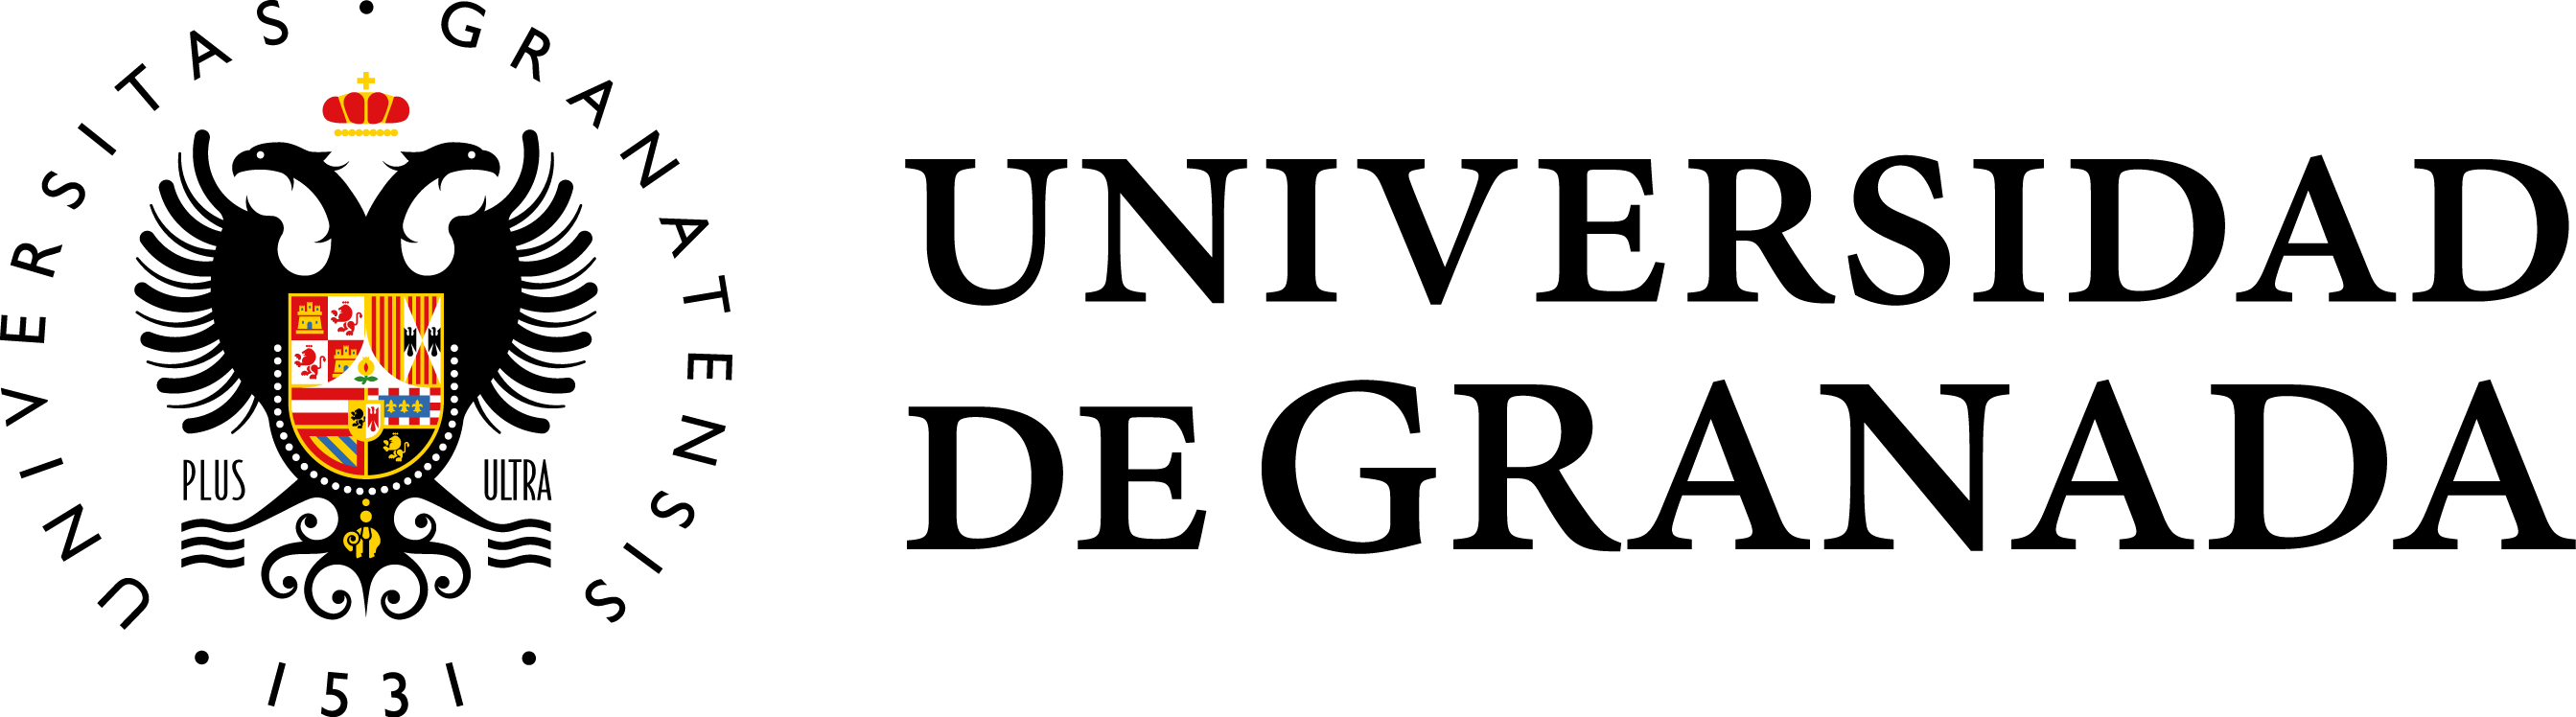
\includegraphics[width=0.8\textwidth]{logo-ugr}
  \caption{Logotipo de la Universidad de Granada}
  \label{fig:logo-ugr}
\end{figure}

\section{Entornos matemáticos}

\begin{teorema}\label{thm:teorema}
Esto es un ejemplo de teorema.
\end{teorema}

\begin{proposicion}
Ejemplo de proposición
\end{proposicion}

\begin{lema}
Ejemplo de lema
\end{lema}

\begin{corolario}
Ejemplo de corolario
\end{corolario}

\begin{definicion}
Ejemplo de definición
\end{definicion}

\begin{observacion}
Ejemplo de observación
\end{observacion}

Y esto es una referencia al \autoref{thm:teorema}. 

Identidad Pitagórica~\eqref{eq:identidad-pitagorica}\index{Identidad pitagórica}
\begin{equation}\label{eq:identidad-pitagorica}
  \cos^2 x + \sin^2 x = 1
\end{equation}

La fórmula de Gauss-Bonnet\index{Gauss-Bonnet!fórmula} para una superficie compacta $S$ viene dada por:
\begin{equation}
  \int_S K = 2\pi\chi(S)
\end{equation}


\section{Bibliografía e índice}

Además incluye varias entradas al índice alfabético mediante el comando \verb+\index+ \index{Leonard!Euler|textbf}


\endinput
